% !TEX TS-program = pdflatex
% !TEX encoding = UTF-8 Unicode

% This is a simple template for a LaTeX document using the "article" class.
% See "book", "report", "letter" for other types of document.

% TODO: Ich habe eventuell irgendwo geschrieben, dass in Haskell kein Ad-Hoc-Polymorphismus benutzt
% wird, was ja Quatsch ist, da das ja gerade der Zweck von Typklassen ist.

\documentclass[11pt]{article} % use larger type; default would be 10pt

\usepackage[utf8]{inputenc} % set input encoding (not needed with XeLaTeX)

\usepackage{todonotes}
\usepackage{mathrsfs}
\usepackage{graphicx}
\usepackage{minted}
\usepackage{url}

%%% Examples of Article customizations
% These packages are optional, depending whether you want the features they provide.
% See the LaTeX Companion or other references for full information.

%%% PAGE DIMENSIONS
\usepackage{geometry} % to change the page dimensions
\geometry{a4paper} % or letterpaper (US) or a5paper or....
% \geometry{margin=2in} % for example, change the margins to 2 inches all round
% \geometry{landscape} % set up the page for landscape
%   read geometry.pdf for detailed page layout information

\usepackage{graphicx} % support the \includegraphics command and options

\usepackage{courier}
\usepackage{amsmath}

\usepackage[ngerman]{babel}

% \usepackage[parfill]{parskip} % Activate to begin paragraphs with an empty line rather than an indent

%%% PACKAGES
\usepackage{booktabs} % for much better looking tables
\usepackage{array} % for better arrays (eg matrices) in maths
\usepackage{paralist} % very flexible & customisable lists (eg. enumerate/itemize, etc.)
\usepackage{verbatim} % adds environment for commenting out blocks of text & for better verbatim
\usepackage{subfig} % make it possible to include more than one captioned figure/table in a single float
% These packages are all incorporated in the memoir class to one degree or another...

\usepackage{amssymb}

%%% HEADERS & FOOTERS
\usepackage{fancyhdr} % This should be set AFTER setting up the page geometry
\pagestyle{fancy} % options: empty , plain , fancy
\renewcommand{\headrulewidth}{0pt} % customise the layout...
\lhead{}\chead{}\rhead{}
\lfoot{}\cfoot{\thepage}\rfoot{}

%%% SECTION TITLE APPEARANCE
\usepackage{sectsty}
\allsectionsfont{\sffamily\mdseries\upshape} % (See the fntguide.pdf for font help)
% (This matches ConTeXt defaults)

%%% ToC (table of contents) APPEARANCE
\usepackage[nottoc,notlof,notlot]{tocbibind} % Put the bibliography in the ToC
\usepackage[titles,subfigure]{tocloft} % Alter the style of the Table of Contents
\renewcommand{\cftsecfont}{\rmfamily\mdseries\upshape}
\renewcommand{\cftsecpagefont}{\rmfamily\mdseries\upshape} % No bold!

%%% END Article customizations

%%% The "real" document content comes below...

\title{Anfang}
\author{Thomas Rossow}
%\date{} % Activate to display a given date or no date (if empty),
         % otherwise the current date is printed 

\begin{document}
\tableofcontents 
\maketitle


% % % % % % % % % % % % % % % % % % % % % % % % % % % % % % % % % % % % % % % % %
\section{Einleitung}
% % % % % % % % % % % % % % % % % % % % % % % % % % % % % % % % % % % % % % % % %

\label{sec:einleitung}

Das Typsystem einer Programmiersprache hat einen erheblichen Einfluss darauf, wie sich die Arbeit mit dieser
Sprache gestaltet. Natürlich wird man jedes Programm, das mit einem statischen Typsystem entwickelt wurde,
auch mit dynamischen Typen schreiben können. Dennoch bietet statische Typsicherheit deutliche Vorteile --
nicht nur während der Entwicklung. Ein Vorteil ist die Möglichkeit, wertvolle Erkenntnisse allein aus den verwendeten
Typen des Programms zu ziehen. Und genau das ist ein zentrales Thema dieser Arbeit.
%Natürlich kann man mit einer streng statisch getypten Sprache nichts entwickeln, das man nicht
%auch mit einem dynamischen Typsystem programmieren kann. Dennoch bietet statische Typisierung nicht nur beim Programmieren
%selbst unbestreitbare Vorteile.

Haskell ist eine funktionale Programmiersprache mit einem statischen Typ\-sys\-tem. Wie es bei vielen funktionalen
Programmiersprachen der Fall ist, basiert auch Haskells Typsystem auf dem Hindley/Milner System \cite{hindley, milner}, was es
Haskell ermöglicht, zu jedem Ausdruck automatisch eine Typsignatur herzuleiten, die den allgemeinsten Typ dieses Ausdrucks
darstellt \cite{wadler}.

Und das ist der Grundsatz: \textit{Jeder} Ausdruck hat einen ganz bestimmten Typ. Dieser Typ steht fest und wird sich auch während der Programmausführung
nicht ändern. Kann ein solcher Typ nicht hergeleitet werden, dann kompiliert das Programm gar nicht erst.
%Jeder Ausdruck in Haskell hat einen ganz bestimmten Typen, und wenn dieser Typ nicht passt, dann kompiliert auch
%das Programm nicht.

Der offensichtliche Vorteil für den Entwickler ist, dass viele unerwünschte Programmzustände gar nicht erst auftreten,
weil sie bereits durch Typfehler abgefangen werden, während eine Programmiersprache mit dynamischem Typsystem solche
Probleme ohne Fehlermeldung durchwinken würde, was nicht selten schwer nachvollziehbare Laufzeitfehler zur Folge hat.
Betrachten wir zum Beispiel die folgende Funktion der Skriptsprache \textit{Javascript} \cite{javascript}.

\begin{minted}{javascript}
function sum(a, b)
{
   return a + b;
}
\end{minted}

Javascript hat ein dynamisches Typsystem, das heißt es können beim Aufruf der Funktion \texttt{sum} Parameter beliebiger Typen
übergeben werden. Ein Laufzeitfehler tritt dann auf, wenn zwei Werte \texttt{a} und \texttt{b} übergeben werden, auf die
der Operator \texttt{+} nicht angewandt werden kann (ein Beispiel hierfür wären Funktionen). Problematisch ist auch der Fall, in
dem zwei Parameter übergeben werden, auf die der \texttt{+}-Operator zwar angewandt werden kann, jedoch nicht das erwartete
Ergebnis liefert. Ein Aufruf von \texttt{sum("42", 7)} würde beispielsweise zum Ergebnis \texttt{"427"} führen.

%Außerdem kann der Entwickler in Haskell
Trotz automatisch hergeleiteten Typen bietet Haskell dem Entwickler zusätzlich die Möglichkeit, zu jedem Ausdruck eine eigene
Typsignatur anzugeben. Das führt nicht dazu,
dass Haskell Ausdrücke auf einmal als völlig andere Typen interpretiert. Vielmehr bedeutet das, dass Haskell Typen, die der
Benutzer manuell angegeben hat, ebenfalls akzeptiert, sofern es sich dabei um Spezialisierungen des allgemeinsten Typs handelt\footnote{Manchmal können Typannotationen einen Unterschied machen, beispielsweise in Verbindung mit Typklassen.}.

Das bietet vor allem den Vorteil, dass Haskell weiß, was der Entwickler erwartet. Es ist durchaus möglich, dass Haskell trotz eines
Denkfehlers des Entwicklers einen Typ herleiten kann, der zur Funk\-tions\-de\-kla\-rati\-on passt -- mit dem man aber nicht rechnet.
Das folgende Beispiel soll veranschaulichen, wie ein solcher Fehler zustande kommen kann.

\begin{minted}{haskell}
concatStrings a b = a : b
\end{minted}

Die angegebene Funktion soll zwei Zeichenketten konkatenieren, verwendet aber statt des Konkatenationsoperators \texttt{++} fälschlicherweise den
Listenkonstruktor \texttt{:}. Das hat zur Folge, dass Haskell als ersten Parameter $a$ ein Listenelement statt einer Liste erwartet,
es ergeben sich jedoch keine Probleme mit der Typsignatur. Problematisch wird es erst, wenn versucht wird, die Funktion
aufzurufen, beispielsweise mit dem folgenden Aufruf, wobei \texttt{b} eine Zeichenkette ist.

\begin{minted}{haskell}
concatStrings "Student#" b
\end{minted}

Haskell erkennt, dass der
Funktionsaufruf nicht mit der (automatisch ermittelten) Funktionssignatur kompatibel ist und erzeugt einen Kompilierfehler. Die
Fehlermeldung besagt allerdings, dass der Typ \texttt{[Char]} nicht mit dem erwarteten Typ \texttt{Char} übereinstimmt
und gibt als Fehlerposition den Funktionsaufruf an.

Hätte der Entwickler die erwartete Typsignatur \texttt{[Char] -> [Char] -> [Char]} angegeben, dann hätte bereits die Typsignatur
einen Fehler erzeugt, da sie kein Spezialfall der automatisch hergeleiteten Signatur \texttt{a -> [a] -> [a]} ist. Zusammenfassend kann man sagen, dass das Typsystem ein wichtiger Faktor bezüglich Fehleranfälligkeit und -prävention ist.
%Durch Typsignaturen hat Haskell jedoch einen Anhaltspunkt, was der Entwickler erwartet. Es ist ja durchaus
%möglich, dass Haskell trotz eines Denkfehlers des Entwicklers einen Typen herleiten kann, der auf die Funk\-tions\-de\-kla\-rati\-on passt, mit dem man aber nicht rechnet.
%Das Typsystem ist also ein wichtiger Faktor bezüglich Fehleranfälligkeit und -prävention.

%eigene Typsignaturen angeben und erhält sofort einen Typfehler, wenn die tatsächlich inferierten Typen nicht mit den
%erwarteten Typsignaturen übereinstimmen. Das Typsystem ist also ein wichtiger Faktor bezüglich Fehleranfälligkeit und
%-prävention.
Besonders vorteilhaft ist Haskells Typsystem aber, um Schlüsse aus Funk\-tions\-sig\-na\-tu\-ren zu ziehen. Betrachtet man eine solche Signatur, offenbart sich oft schon ein Teil der Funktionalität, da die
Einschränkungen des Typsystems wenig Spielraum für unerwartetes Verhalten lassen. Die folgende Zeile zeigt ein Beispiel
für eine solche Funktionstypsignatur.
%
%Die funktionale Programmiersprache Haskell bietet ein komplexes Typsystem, das auf der Typinferenz nach Hindley-Milner basiert \todo{cite}.
%Zu jedem Ausdruck lässt sich eine Typsignatur herleiten, die den allgemeinsten Typen dieses Ausdrucks darstellt. Außerdem
%kann der Programmierer zu jedem Ausdruck eine Typsignatur angeben, was zur Übersicht beiträgt und Fehlern vorbeugt.
%Das Typsystem ist so mächtig, dass die Typsignatur allein schon sehr viele Rückschlüsse über die zugehörige Funktion ermöglicht.
%Betrachten wir beispielhaft die folgende Signatur.

\begin{minted}{haskell}
applyOnList :: (a -> b) -> [a] -> [b]
\end{minted}

Es handelt sich um eine Funktion namens \texttt{applyOnList}, die als ersten Parameter eine Funktion erwartet, die einen beliebigen
Typ auf einen anderen (oder den gleichen) beliebigen Typ abbildet. Beim zweiten Parameter muss es sich um eine Liste handeln,
deren Listenelemente vom Typ $a$ sind, also vom Typ, den die als erster Parameter übergebene Funktion als
Eingabewert erwartet.

Allein durch diesen Typ lässt sich bereits erahnen, was sich ungefähr hinter dieser Funktion verbirgt.
Es ist anzunehmen, dass die  Funktion \texttt{applyOnList} die Eingabeliste mithilfe der übergebenen Funktion manipuliert und die
resultierende Liste zurückgibt. Natürlich ist es nicht gesagt, dass sie das tut, es drängt sich aber die Annahme auf, dass sie
etwas ``Ähnliches'' tun muss -- einfach deshalb, weil es der Typ suggeriert.
%Natürlich kann man nicht einfach davon ausgehen, dass die Funktion in ihrer Implementierung die Funktion des ersten Parameters
%auf jedes Listenelement des zweiten Parameters anwendet und das Ergebnis zurückgibt, aber eine ähnliche Funktionsweise
%ist zu erwarten - einfach aus dem Grund, dass die Funktion ``nicht viel anderes'' mit den gegebenen Typen machen kann.

Haskell stellt in der Prelude\footnote{Die Prelude ist Haskells Standardbibliothek, die automatisch importiert wird \cite{haskell}.}
eine Funktion \texttt{map} bereit, die die gleiche Signatur wie unsere Beispielfunktion \texttt{test} hat. Und \texttt{map} macht tatsächlich genau das, was
man erwarten würde: Es wendet die übergebene Funktion auf jedes Element der übergebenen Liste an und liefert die Ergebnisliste.
%Haskell liefert eine solche Funktion in der , man kennt sie unter dem Namen \texttt{map}.
Dass sich \texttt{test} und
\texttt{map} eine Typsignatur teilen, lässt Rückschlüsse auf eine ähnliche Funktionsweise zu. Dass diese Ähnlichkeit
nicht auf vage Mutmaßungen beschränkt ist, sondern dass sogar ganz systematisch konkrete Aussagen zu beliebigen Typsignaturen
hergeleitet werden können, ist Thema der sogenannten \textit{freien Theoreme}, auf die in Kapitel \ref{sec:freie-theoreme}
genauer eingegangen wird.
%das wird thematisiert in Kapitel \ref{sec:freie-theoreme}, in dem es um die sogenannten
%\textit{freien Theoreme} geht - Aussagen, die sich für beliebige Typsignaturen herleiten lassen.

Da die Herleitung dieser freien Theoreme ganz systematisch und immer gleich abläuft, kann sie auch ohne Probleme
programmatisch erledigt werden. Das Haskell-Paket \textit{free-theorems} \cite{freetheorems} enthält eine Bibliothek, die
genau diese Aufgabe erledigt, und für die sogar eine Weboberfläche existiert \cite{freetheoremswebui}.
Diese Bibliothek ermöglicht es, Haskell-Code einzulesen und aus beliebigen Typsignaturen die entsprechenden freien
Theoreme zu generieren, wobei sogar eigene Datentypen in den Signaturen verwendet werden können.
%Die Weboberfläche geht sogar noch einen Schritt weiter und kennt bereits eine Reihe wichtiger Deklarationen aus der Haskell-Prelude.
Die Web\-ober\-flä\-che enthält darüber hinaus  eine Liste bekannter Deklarationen aus der Prelude.

%Die Herleitung freier Theoreme ist so generisch, dass sie auch programmtisch erledigt werden kann. Genau das macht
%\cite{bla} \todo{cite} - hierbei handelt es sich um die Bibliothek \textit{free-theorems}, die es ermöglicht, Haskell-Code einzulesen
%und aus beliebigen Typsignaturen Formeln zu generieren, die die entsprechenden freien Theoreme repräsentieren. Zudem gibt es
%mit \cite{x} \todo{cite} eine Webanwendung, die einen Zugriff auf die Funktionen der Bibliothek ermöglicht.
%Leider bietet die Bibliothek \textit{free-theorems} nicht sämtliche Sprachfunktionen von Haskell an. 

Neben algebraischen Datentypen ist es in Haskell auch möglich, eigene Typklassen zu definieren und in
Typsignaturen zu verwenden. Ein prominentes Beispiel für eine Typklasse ist \texttt{Eq}. Dabei handelt es sich um
die Klasse der vergleichbaren Datentypen, die den Gleichheitsoperator \texttt{==} definiert.

Allein in der Prelude sind Typklassen allgegenwärtig, da sie mit Ad-Hoc-Poly\-mor\-phis\-mus ein mächtiges Werkzeug bieten,
um Programme zu strukturieren. Die Bibliothek \textit{free-theorems} unterstützt die Verwendung von Typklassen. Es ist möglich, eigene
Klassen zu deklarieren und freie Theoreme aus Typsignaturen zu generieren, in denen Typklassen verwendet werden.
%Typklassen sind ein praktisches Sprachelement von Haskell, weshalb es sinnvoll ist,
%dass sie von \textit{free-theorems} unterstützt werden.

Allerdings unterstützt die Bibliothek lediglich Typklassen für Datentypen, die keine Typparameter haben. Haskell erlaubt es,
Datentypen zu definieren, die Typen als Parameter erwarten. Haskell erlaubt es ebenso, Typklassen für parametrisierte
Datentypen zu deklarieren. Dass es sich dabei nicht um eine unwichtige Kleinigkeit im Sprachumfang von Haskell handelt, wird spätestens klar, wenn man
sich in Erinnerung ruft, dass auch die bekannte Typklasse \texttt{Monad} eine Typkonstruktorklasse ist, die in Haskell sehr häufig
Anwendung findet.

Es ist also wünschenswert, \textit{free-theorems} derart zu erweitern, dass es auch mit Typkonstruktorklassen zurecht kommt und
freie Theoreme für entsprechende Typsignaturen generieren kann. Und genau darauf liegt der Fokus dieser Arbeit. Es wird
erläutert, wie die Bibliothek und insbesondere die Anpassungen für Typkonstruktorklassen aussehen.

Dazu wird in Kapitel \ref{sec:grundlagen} zunächst auf die mathematischen Grundlagen eingegangen, also Notationen, Definitionen,
etc., die für das Verständnis der daraufhin folgenden Abschnitte benötigt werden.
Die allgemeine Herangehensweise zum Herleiten freier Theoreme ist dann das Thema von Kapitel \ref{sec:freie-theoreme}, in dem
das sogenannte \textit{Parametrizitätstheorem} eingeführt wird, das dann zu freien Theoremen führt.
Am Ende des Kapitels geht es dann um die Erweiterung der Theorie auf Typkonstruktorklassen. Um die Anwendbarkeit dieser
Theorie zu motivieren, werden daraufhin einige Anwendungsbeispiele gegeben.

%Dazu wird zunächst auf die
%Grundlagen eingegangen, die benötigt werden, um die Theorie dahinter zu verstehen. Im folgenden Abschnitt geht es um das
%allgemeine Vorgehen beim Herleiten freier Theoreme. Insbesondere wird dabei auch auf Typkonstruktorklassen eingegangen.

%Ein wichtiger Aspekt
%bei der Programmierung in Haskell sind Typklassen. Sie ermöglichen es, Datenstrukturen in Klassen einzuordnen, und für diese
%Klassen Funktionen anzugeben, die pro Datentyp implementiert werden können. Kurz gesagt erlauben Typklassen Ad-Hoc-Polymorphismus in Haskell.

%Zwar unterstützt die Bibliothek Typklassen, allerdings nur für Datentypen, die keinen Typen als Parameter erwarten. Die
%bekanntere \texttt{Monad}-Klasse beispielsweise ist für Datentypen definiert, die einen Typparameter haben. Eine Verwendung
%mit der \texttt{free-theorems} Bibliothek ist somit nicht möglich, oftmals möchte man aber nicht auf solche Typklassen verzichten.
%Grundsätzlich unterscheidet sich die Verwendung von Typkonstruktorklassen gar nicht gravierend von einfachen Typklassen.

%Ich habe die Bibliothek um eine entsprechende Funktionalität erweitert. In der vorliegenden Arbeit wird erläutert, wie die Bibliothek
%und insbesondere die Anpassungen für Typkonstruktorklassen aussehen. Dazu wird zunächst auf die Grundlagen eingegangen,
%die benötigt werden, um die Theorie dahinter zu verstehen. Im folgenden Abschnitt geht es um das allgemeine Vorgehen beim
%Herleiten freier Theoreme. Insbesondere wird dabei auch auf Typkonstruktorklassen eingegangen.

Schließlich wird in Kapitel \ref{sec:free-theorems} die Bibliothek \textit{free-theorems} etwas genauer beschrieben, wobei
insbesondere auf den Aufbau und die grundsätzliche Aufteilung eingegangen wird. Die nötigen Anpassungen für die Erweiterung um
Typkonstruktorklassen sind dann in Kapitel \ref{sec:erweiterung-um-typklassen} zu finden.
%um dann im darauf folgenden Abschnitt zu erläutern, an welchen Stellen diese
%Bibliothek erweitert werden muss, um die zusätzliche Funktionalität für Typkonstruktorklassen zu leisten.

In dieser Arbeit wird dabei größtenteils von einer vereinfachten Teilsprache von Haskell ausgegangen, die weder Striktheit noch den Fixpunktoperator kennt. Das reicht nicht aus, um alle realen Haskell-Programme zu beschreiben, und in Kapitel \ref{sec:striktheit-und-rekursion}
wird genauer darauf eingegangen, welche Konzepte in dieser Teilsprache fehlen und wie sie von \textit{free-theorems} behandelt
werden.
%In dieser Arbeit wird dabei größtenteils von einer vereinfachten Teilsprache von Haskell ausgegangen, die weder Striktheit noch
%den Fixpunktoperator kennt. Natürlich entspricht dies nicht immer den realen Begebenheiten, und die Bibliothek
%\texttt{free-theorems} berücksichtigt dies bereits, indem sie unterschiedliche Teilsprachen anbietet, die die entsprechenden
%Sprachfunktionen berücksichtigen. Die Erweiterungen für Typkonstruktorklassen berücksichtigen diese Problematik derzeit noch
%nicht. Kapitel \ref{sec:striktheit-und-rekursion} geht genauer darauf ein, inwiefern \texttt{seq} und \texttt{fix} in Verbindung
%mit freien Theoremen problematisch sind.

Am Ende der Arbeit findet sich schließlich ein zusammenfassendes Kapitel und ein Ausblick, der Anstöße für zukünftige Arbeiten
liefert.

%Die eingeführten Erweiterungen für Typkonstruktorklassen gehen von einer Basissprache ohne diese Besonderheiten aus.
%In Abschnitt \ref{sec:striktheit-und-rekursion} wird kurz erläutert, welche Auswirkungen diese Besonderheiten haben, in der
%Implementierung sind sie noch nicht vorgesehen - hier ist noch Raum für Erweiterungen. \todo{würde man das hier schreiben?}

% % % % % % % % % % % % % % % % % % % % % % % % % % % % % % % % % % % % % % % % %
\section{Grundlagen}
% % % % % % % % % % % % % % % % % % % % % % % % % % % % % % % % % % % % % % % % %

% TODO: id_{M} ist die Relation, in der alle Elemente der Menge M mit sich selbst verwandt sind.

\label{sec:grundlagen}

Bevor auf die eigentliche Thematik eingegangen wird, bietet es sich an, einige Grundlagen zu klären, die im Laufe dieser Arbeit
von Bedeutung sein werden. Ein großer Teil der Arbeit baut auf dem mathematischen Konstrukt der Relation auf, weshalb neben
grundsätzlichen mathematischen Notationen vor allem Definitionen und Notationen eingeführt werden, die Relationen betreffen.

Des Weiteren sind Haskell-Kenntnisse erforderlich für das Verständnis der weiteren Arbeit. Es würde an dieser Stelle zu weit führen, sämtliche Sprachkonstrukte von
Haskell anzuführen, die für die folgenden Abschnitte von Bedeutung sind; dennoch wird zumindest auf Typklassen eingegangen, insbesondere Typkonstruktorklassen,
da diese für die Arbeit eine signifikante Rolle spielen. Zudem bietet es sich an, von Anfang an einige Benennungen einzuführen, die im Laufe der
Arbeit immer wieder auftauchen werden.

%Sämtliche sprachliche Konstrukte von
%Haskell zu erläutern, die im Laufe dieser Arbeit erscheinen, würde an dieser Stelle zu weit führen. Es wird aber auf das Konstrukt
%der Typklassen, insbesondere der Typkonstruktorklassen, eingegangen, da diese im weiteren Verlauf der Ausarbeitung eine
%signifikante Rolle spielen. Zudem bietet es sich an, von Anfang an einige Benennungen einzuführen, die im Laufe der Arbeit
%immer wieder gebraucht werden.

%Es soll hier nicht darum gehen,
%die komplette Programmiersprache Haskell zu beschreiben, aber es wird auf das Konzept der Typkonstruktorklassen eingegangen, da diese
%in dieser Ausarbeitung eine gesonderte Rolle spielen.

%In diesem Abschnitt sollen einige Grundlagen eingeführt werden, die in den folgenden Kapiteln von Bedeutung sind. Zunächst werden
%einige mathematische Definitionen und Notationen angegeben, die zum großen Teil Relationen betreffen.
%Daraufhin wird noch einmal kurz auf Typklassen in Haskell eingegangen.

%Da diese Arbeit zu großen Teilen auf \cite{freetheorems} aufbaut, werden die dort verwendeten Notationen größtenteils
%weiter verwendet.

%Die mathematischen Notationen in diesem Kapitel halten sich größtenteils an die Darstellungen von Böhme in \cite{freetheorems}

%Die in diesem Abschnitt
%eingeführten Notationen orientieren sich größtenteils an den Definitionen aus \cite{freetheorems}.

%Die Notationen, die hier eingeführt werden, bauen größtenteils auf \cite{freetheorems} auf, da die dort beschriebene Bibliothek
%die Grundlage für die vorliegende Arbeit darstellt.


% % % % %% % % % % % % % % % % %


% - - - - - - - - - - - - - - - - - - - - - - - - - - - - - - - - - - - - - - - - - - - - - - - - - - - - - - - - - - - - - - - - - - - - - - - - - - - - - -
\subsection{Relationen}
% - - - - - - - - - - - - - - - - - - - - - - - - - - - - - - - - - - - - - - - - - - - - - - - - - - - - - - - - - - - - - - - - - - - - - - - - - - - - - -

%\begin{mydef}
%Ist $X$ eine Menge, dann ist durch $\mathcal{P}(X)$ die Potenzmenge von $X$ gegeben, bei der es sich um die Menge handelt, die alle Teilmengen von $X$ beinhaltet, d.h. $\mathcal{P}(X) = \{ T~|~ T \subseteq X\}$.
%\end{mydef}

Die mathematische Grundlage und das wichtigste Werkzeug beim Erzeugen von freien Theoremen sind Relationen.

%Sie werden im Zusammenhang mit freien Theoremen verwendet, um Ausdrücke einander zuzuordnen, die durch Polymorphie einander
%ähnlich bzw. ``austauschbar'' sind.

\begin{mydef}
Eine \textit{binäre Relation} ist auf zwei Mengen definiert, deren Elemente sie einander zuordnet. Die Schreibweise
$\mathcal{R} : T_1 \Leftrightarrow T_2$ sagt, dass $\mathcal{R} \subseteq T_1 \times T_2$ eine auf den Mengen $T_1$ und $T_2$ definierte
Relation ist.
\end{mydef}

Man kann die Relation als eine Menge von Paaren auffassen, wobei jedes Paar aus einem Element aus $T_1$ und einem
Element aus $T_2$ besteht.
Die Aussage $(x, y) \in \mathcal{R}$ bedeutet also, dass $x$ und $y$ bezüglich $\mathcal{R}$ verwandt sind. Man schreibt hierfür
gelegentlich auch $x\ \mathcal{R}\ y$ (hauptsächlich, wenn es sich bei $\mathcal{R}$ um ein Operatorsymbol handelt).
Anders ausgedrückt ordnet eine Relation jedem Element aus der ersten Menge beliebig viele Elemente aus der zweiten Menge zu.

Eine besondere Relation, die sich aus einer beliebigen Menge erzeugen lässt, ist die sogenannte \textit{Identitätsrelation}, die
auch in freien Theoremen eine wichtige Rolle spielt.

\begin{mydef}
Ist $M$ eine Menge, so bezeichnet $id_{M}$ die \textit{Identitätsrelation} auf dieser Menge, die definiert ist durch
$id_{M} = \{ (x, x) | x \in M \}$, in der also jedes Element aus $M$ mit sich selbst verwandt ist.
\end{mydef}

Ein Beispiel für Identitätsrelationen lässt sich ganz einfach für die Menge $\mathcal{B}$ der Wahrheitswerte geben. Es ist
$\mathcal{B} = \{ tt, ff \}$, somit ist $id_{\mathcal{B}} = \{ (tt, tt), (ff, ff) \}$.
%Erfüllen Relationen bestimmte Gesetzmäßigkeiten \todo{?}, kann man sie in bestimmte Relationen unterteilen, so zum Beispiel
%\textit{partielle Ordnungen}.
Man kann die Menge der Relationen weiter unterteilen, ein Spezialfall der Relation ist beispielsweise die \textit{partielle Ordnung}.

\begin{mydef}
Eine partielle Ordnung $\sqsubseteq : M \Leftrightarrow M$ ist eine Relation, die \textit{reflexiv}, \textit{antisymmetrisch} und \textit{transitiv} ist, d.h. es gelten die folgenden Aussagen für alle $x, y, z \in M$.
\begin{align*}
& x \sqsubseteq x & \text{(Reflexivität)} \\
& x \sqsubseteq y \land y \sqsubseteq x \Rightarrow x = y & \text{(Antisymmetrie)} \\
& x \sqsubseteq y \land y \sqsubseteq z \Rightarrow x \sqsubseteq z & \text{(Transitivität)} \\
\end{align*}
\end{mydef}

Als Beispiel für eine solche partielle Ordnung lässt sich der Teilmengenoperator $\subseteq$ auf beliebigen Mengen betrachten.
Wie man sich leicht klar machen kann, gilt für $\subseteq$ Reflexivität, Antisymmetrie und Transitivität.
%Dass für beliebige Mengen Reflexivität, Antisymmetrie und Transitivität gelten, sollte klar sein und wird hier nicht weiter
%vertieft \todo{vielleicht anders schreiben}.

In Abschnitt \ref{sec:striktheit-und-rekursion} wird eine partielle Ordnung genutzt, um Ausdrücke bezüglich ihrer \textit{Definiertheit}'
zu ordnen. Dazu müssen einige zusätzliche Definitionen eingeführt werden,
um partielle Ordnungen weiter einzuschränken. Die folgenden
Definitionen richten sich dabei nach Johann und Voigtländer \cite{johann2006}.

\begin{mydef}
Wenn $\sqsubseteq_{X}$ ein kleinstes Element besitzt, dann ist $\sqsubseteq_{X}$ eine komplette Partialordnung und man nennt $X$
\textit{geordnet}. Dieses kleinste Element wird typischweise als $\bot_{X}$ (\textit{bottom}) bezeichnet, wobei man den Index
auch weglassen kann, wenn klar ist, welche Menge gemeint ist.
\end{mydef}

\begin{mydef}
Sei $\mathcal{R} \subseteq X \times Y$ eine binäre Relation über zwei geordneten Mengen $X$ und $Y$. Man nennt $\mathcal{R}$ \textit{strikt},
wenn $(\bot, \bot) \in \mathcal{R}$. $\mathcal{R}$ wird \textit{total} genannt, wenn für jedes Paar $(x, y) \in \mathcal{R}$ gilt, dass
aus $y = \bot$ folgt $x = \bot$.
\end{mydef}

\begin{mydef}
Man nennt $\mathcal{R}$ \textit{bottom-reflexiv}, wenn für jedes Paar
$(x, y) \in \mathcal{R}$ gilt: $y = \bot \Leftrightarrow x = \bot$.
\end{mydef}

Schließlich soll \textit{Stetigkeit} eingeführt werden, wozu zunächst die Definition einer \textit{monotonen Sequenz} benötigt wird.

\begin{mydef}
Sei X eine Menge und $\sqsubseteq_{X}$ eine partielle Ordnung über X. Man nennt eine Funktion $\bar{x} : \mathbb{N} \rightarrow X$
eine \textit{monotone Sequenz} über $X$, wenn $\bar{x}(i) \sqsubseteq_{X} \bar{x}(i + 1)$ für alle $i \in \mathbb{N}$.
\end{mydef}

Anders ausgedrückt ist eine monotone Sequenz also eine Menge von Elementen einer Ordnung,
die jeder natürlichen Zahl ein Element aus der geordneten Menge
zuordnet, sodass eine Erhöhung der Zahl auch eine Erhöhung des Elements bezüglich der Ordnung zur Folge hat.
Auf dieser Definition von monotonen Sequenzen aufbauend lässt sich nun eine Definition für \textit{Stetigkeit} formulieren, darüber
hinaus nennen wir die Kombination aus Stetigkeit und Striktheit \textit{zulässig}.

\begin{mydef}
Wenn für alle monotonen Sequenzen $\bar{x}$ über $X$ und $\bar{y}$ über $Y$, die die Aussage $(\bar{x}(i),~\bar{y}(i)) \in\mathcal{R}$
erfüllen, jeweils das Paar der Suprema ($\bigsqcup{\bar{x}}, \bigsqcup{\bar{y}})$ ebenfalls in $\mathcal{R}$ ist, dann nennt man $\mathcal{R}$ \textit{stetig}.
\end{mydef}

\begin{mydef}
Eine Relation ist \textit{zulässig}, wenn sie strikt und stetig ist.
\end{mydef}

Hat man zwei Relationen gegeben, lassen sich aus diesen neue Relationen konstruieren, beispielsweise durch die Relationskomposition.

\begin{mydef}
Sind drei Mengen $X$, $Y$ und $Z$ und zwei binäre Relationen $\mathcal{R} : X \Leftrightarrow Y$ und $\mathcal{R} : Y
\Leftrightarrow Z$ gegeben, dann definiert man die \textit{Komposition} von $\mathcal{R}$ und $\mathcal{S}$,
geschrieben $\mathcal{R} ; \mathcal{S}$, wie folgt.
\begin{align*}
\mathcal{R} ~;~ \mathcal{S} = \{ (x, z) ~|~ \exists y \in Y .~ (x, y) \in \mathcal{R} \wedge (y, z) \in \mathcal{S} \} \subseteq X \times Z
\end{align*}
\end{mydef}

In Worten ausgedrückt bedeutet das, dass man zwei Relationen zu einer neuen Relation zusammenfügt, in der zwei Elemente
$x$ und $z$ verwandt sind, wenn es ein Bindeelement $y \in Y$ gibt, mit dem das erste Element $x$ in der ersten Relation und das
zweite Element $z$ in der zweiten Relation verwandt ist.

Wir betrachten ein Beispiel, in dem die folgenden Mengen und Relationen definiert sind.
\begin{align*}
&M = \{ 1, 2, 3 \}, N = \{ a, b, c \}, O = \{ \alpha, \beta, \gamma \} \\
&\mathcal{R} : M \Leftrightarrow N, \mathcal{S} : N \Leftrightarrow O \\
&\mathcal{R} = \{ (1, a), (2, b), (3, c) \} \\
&\mathcal{S} = \{ (a, \alpha), (b, \beta), (c, \gamma) \}
\end{align*}

Durch Komposition der beiden Relationen $\mathcal{R}$ und $\mathcal{S}$ ergibt sich die folgende Relation.
\begin{align*}
R ; S = \{ (1, \alpha), (2, \beta), (3, \gamma) \}
\end{align*}

Mithilfe von Relationskomposition kann man nun sehr leicht \textit{Linksabgeschlossenheit} definieren.

\begin{mydef}
Ist Y eine Menge und X eine bezüglich $\sqsubseteq_{X}$ geordnete Menge, dann nennt man eine Relation $\mathcal{R} \subseteq X \times Y$ \textit{linksabgeschlossen}, wenn $\sqsubseteq_{X} ; R = R$.
\end{mydef}

Eine Relation $\mathcal{R}$ ist also linksabgeschlossen bezüglich einer Ordnung $\sqsubseteq_{X}$, wenn die Komposition dieser Ordnung mit $\mathcal{R}$
wieder $\mathcal{R}$ ergibt, oder in anderen Worten: wenn für jedes $(x, y) \in \mathcal{R}$ gilt, dass zu jedem $a \sqsubseteq_{X} x$
auch $(a, y) \in \mathcal{R}$.

\begin{mydef}
Das Inverse einer Relation $\mathcal{R} : X \Leftrightarrow Y$ wird definiert als $\mathcal{R}^{-1} = \{(y, x) ~|~ (x, y) \in \mathcal{R}\}
\subseteq Y \times X$. Möchte man $\sqsubseteq^{-1}$ ausdrücken, nutzt man zuweilen auch das umgedrehte Symbol $\sqsupseteq$.
\end{mydef}

\begin{mydef}
Seien $X$ und $Y$ geordnete Mengen und $f : X \rightarrow Y$ eine Funktion. Man nennt $f$ \textit{monoton}, wenn aus $x
\sqsubseteq_{X} y$ folgt, dass $f(x) \sqsubseteq_{Y} f(y)$ für alle $x, y \in X$.
\end{mydef}

%Sei $V$ eine endliche Menge und $\mathcal{E}$ eine binäre Relation auf $V$. Das Tupel $G = (V, \mathcal{E}) bezeichnet einen
%\textit{gerichteten Graphen}. Die Elemente von $V$ nennt man \textit{Vertices}. Die transitive Hülle von $E$ bezeichnet man mit
%$\mathcal{E}^{+}$. Sei $V_c = \{ v \in V | (v, v) } \in \mathcal{E}^{+} \} die Menge aller Vertizes, die Teil eines Kreises sind.
%
%Für je zwei Teilmengen $V_1, V_2 \subseteq V$, bezeichnet die Menge $R(V_1, V_2) = \{ v_2 \in V_2 | \exists v_1 \in V_1. (v_1, v_2) \in
%\mathcal{E}^{+} \} alle Vertices in $V_2$, die von einem Vertex aus $V_1$ aus erreichbar sind.Wenn $V'$ eine Teilmenge von $V$ ist,
%dann ist die Menge $V' \backslash R(V \backslash V', V') 
% % % % % % % % % % % % % % % % %

%\subsubsection{Relationen und Funktionen}
%`````````````````````````````````

Wie bereits erwähnt, ordnet eine Relation einem Element ein einzelnes Element, mehrere Elemente oder gar keine Elemente zu.
Das unterscheidet sie von einer Funktion, oder anders ausgedrückt: Das macht Funktionen zu speziellen Relationen. Eine
Funktion, ebenfalls auf zwei Mengen definiert, ordnet jedem Element genau ein Ergebnis zu -- Eingabewerte mit
mehreren Funktionswerten sind genausowenig enthalten wie Eingabewerte ohne Ergebnis.

Wir betrachten eine beliebige Funktion $f : T_1 \rightarrow T_2$. Zu jedem $x \in T_1$ ist also $f(x)$ definiert, wobei $f(x) \in T_2$. Funktionen kann man auch wie folgt als Relationen darstellen.
\begin{align*}
\{ (x, f(x)) ~|~ x \in T_1 \}
\end{align*}

Man nennt die zu $f$ gehörige Relation auch den \textit{Graphen} zu $f$.
Umgekehrt heißt das natürlich, dass eine Relation unter Umständen auch eine Funktion ist. Das wird besonders interessant, wenn man
über Relationen allquantifiziert, zu sehen im folgenden Beispiel.
\begin{align*}
\forall \mathcal{R} : T_1 \Leftrightarrow T_2 . A(\mathcal{R})
\end{align*}

Hierbei ist $A(\mathcal{R})$ eine Aussage, die von $\mathcal{R}$ abhängt.
Diese Aussage lässt sich verschärfen, indem man statt über Relationen über Funktionen $\forall f : T_1 \rightarrow T_2$ quantifiziert.
Eine Aussage wie  $(x, y) \in \mathcal{R}$ wird dann beispielsweise zu $f\ x = y$.

Man kann sich leicht klar machen, dass eine solche spezialisierte Aussage aus der ursprünglichen Aussage folgt. Gilt die ursprüngliche
Aussage, gilt dementsprechend auch die speziellere Aussage.

%Andererseits bedeutet das, dass es Relationen gibt, die man auch als Funktionen auffassen kann. Hat man beispielsweise
%eine Aussage über beliebige Relationen $\forall \mathcal{R} : T_1 \Leftrightarrow T_2 . A(\mathcal{R})$, wobei A eine
%Aussage ist, die von $\mathcal{R}$ abhängig ist, dann macht es Sinn, aus dieser Aussage eine speziellere Aussage zu folgern,
%die wie folgt aussieht.
%
%\begin{align*}
%\forall f : T_1 \rightarrow T_2 . A'(f)
%\end{align*}
%
%Hierbei ist A'(f) die auf Funktionen spezialisierte Aussage. Aus jeder Aussage über beliebige Relationen folgt also eine
%Aussage über entsprechende Funktionen. Dies ist für freie Theoreme von Bedeutung, da man sich vor allem für eine vereinfachte
%Darstellung mit Funktionen interessiert.


% - - - - - - - - - - - - - - - - - - - - - - - - - - - - - - - - - - - - - - - - - - - - - - - - - - - - - - - - - - - - - - - - - - - - - - - - - - - - - -
\subsection{Haskell}
% - - - - - - - - - - - - - - - - - - - - - - - - - - - - - - - - - - - - - - - - - - - - - - - - - - - - - - - - - - - - - - - - - - - - - - - - - - - - - -

Die in dieser Arbeit verwendete Bibliothek generiert freie Theoreme für in Haskell geschriebene Programme. In diesem Abschnitt wird noch einmal speziell auf das Sprachkonstrukt der Typkonstruktorklassen eingegangen.
Eine generelle Beschreibung der Sprache Haskell würde an dieser Stelle zu weit führen, hier sei auf \cite{haskell} verwiesen.

%In dieser Arbeit wird mit einer Teilsprache von Haskell gearbeitet, die ähnlich funktioniert wie der Girard-Reynolds-Kalkül,
%erweitert um Fixpunkte, algebraische Datentypen und \textit{seq} \cite{johann}. Zu beachten ist, dass keine formelle
%Semantik für die komplette Programmiersprache Haskell existiert \cite{johann}. \todo{nötig?}

%%% SO ZIEMLICH 1:1 AUS WADLER ÜBERNOMMEN %%%
%Haskell basiert auf dem Hindley/Milner Typsystem, in dem Typen nicht explizit angegeben werden müssen, sondern der allgemeinste
%Typ automatisch anhand der Definition inferiert werden kann \cite{wadler}.
%In dieser Arbeit wird, wie auch in \cite{wadler}, das
%Girard/Reynolds System verwendet, in dem die explizite Angabe von Typen gebundener Funktionsvariablen gefordert ist und
%Typapplikation bei polymorphen Typen explizit angezeigt werden muss \cite{wadler}.
%Da jedes Programm im Hindley/Milner System automatisch in das Giraard/Reynolds System überführt werden kann, entstehen hier
%keine Probleme.

%%%



%Der Fokus
%liegt dabei auf der Erweiterung um Typkonstruktorklassen, weshalb in diesem Abschnitt kurz darauf eingegangen werden soll,
%wie genau eine solche Klasse in Haskell definiert wird. Ansonsten wird davon ausgegangen, dass grundsätzliche Kenntnisse der
%Programmiersprache vorhanden sind, andernfalls sei an dieser Stelle auf \cite{haskell} verwiesen.

Typklassen in Haskell ermöglichen die Umsetzung von Ad-Hoc-Polymorphismus. Man kann beliebige Typklassen selbst definieren,
wobei eine Typklasse immer aus einem Namen, beliebig vielen Funktionssignaturen und gegebenenfalls auch aus vordefinierten
Standardimplementierungen einzelner Funktionen besteht. Haskell transformiert Programme, die Typklassen verwenden, intern in Programme
ohne dieses Konstrukt -- man nennt diesen Vorgang auch Wörterbuchtransformation (engl. ``dictionary translation'') \cite{jones}.

Es folgt ein einfaches Beispiel, das auch in der Prelude von Haskell enthalten ist.

%Typklassen in Haskell setzen Ad-Hoc-Polyphormismus um und können beliebig definiert werden. Eine Typklasse besteht aus
%einem Namen, beliebig vielen Funktionssignaturen und gegebenenfalls aus vordefinierten Implementierungen einzelner
%Funktionen. Es folgt ein einfaches Beispiel, das auch in der Prelude von Haskell enthalten ist \todo{ist es?}.

\begin{minted}{haskell}
class Show a where
   show :: a -> String
\end{minted}

Der Name dieser Beispielklasse ist \texttt{Show}. Man gibt eine Typvariable an, in diesem Fall \texttt{a}, die auch in jeder
Funktionssignatur vorkommen muss. In dieser Beispielklasse wird genau eine Funktionssignatur eingeführt: Die Signatur
\texttt{a -> String} für die Funktion \texttt{show}.

Im weiteren Haskellprogramm können nun für beliebige Datentypen Instanzdeklarationen angegeben werden. Der folgende
Quellcode zeigt ein Beispiel für einen selbstdefinierten Datentyp.

\begin{minted}{haskell}
data Test = Test Int String

instance Show Test where
   show (Test _ s) = "Test " ++ s
\end{minted}

Kommt nun im Programm in einem Ausdruck der Funktionsaufruf \texttt{show} vor, so wird anhand des Parametertypen
entschieden, welche Instanz dieser Klasse verwendet wird. Es kann also für jeden Typen eine komplett eigene Implementierung
angegeben werden.

Hat man eine Typklasse definiert, kann man im Folgenden in beliebigen Typsignaturen einen Kontext angeben, der
bestimmte Typvariablen auf bestimmte Klassen festlegt, wie es das folgende Beispiel zeigt.

\begin{minted}{haskell}
test :: Functor f => f Int -> f Int
\end{minted}

Hier ist \texttt{f} eine freie Typvariable, für die jedoch ein Kontext angegeben ist, der besagt, dass für $f$ nur Instanzen
der Typklasse \texttt{Functor} infrage kommen. Im Gegenzug für diese Einschränkung ist es in der Implementierung möglich,
die Funktionen dieser Klasse mit dieser Variable zu nutzen, da sichergestellt ist, dass Implementierungen dieser Funktionen
existieren. Die folgende Funktionsdefinition ist also eine mögliche Implementierung der obigen Beispielsignatur.

\begin{minted}{haskell}
test x = fmap (+1) x
\end{minted}

Haskell erkennt, dass \texttt{x} ein Typ sein muss, für den eine \texttt{Functor}-Instanz deklariert ist, weshalb eine
\texttt{fmap}-Implementierung existiert.

Nun ist es ja auch möglich, dass ein selbstdefinierter Datentyp einen Typ als Parameter erwartet, wie das folgende Beispiel
zeigt.

\begin{minted}{haskell}
data Test a = Test a String
\end{minted}

Beim Ausdruck \texttt{Test} handelt es sich in diesem Fall also nicht um einen Typ, sondern eher um einen funktionsähnlichen Ausdruck, der
einen Typ als Parameter erwartet und einen Typ zurückgibt. Man spricht hier auch von \textit{Sorten} (engl. ``kinds''). Haskell
führt für Sorten eine eigene Notation ein. Alle Basistypen wie \texttt{Int}, \texttt{String}, etc. sind von der Sorte *.
Typkonstruktoren, die einen Typen als Parameter erwarten und daraus einen neuen Typen konstruieren, sind von der Sorte
$* \rightarrow *$.
Kompliziertere Sorten wie zum Beispiel $* \rightarrow (* \rightarrow *) \rightarrow *$ sind theoretisch ebenfalls möglich,
werden aber in dieser Arbeit keine Anwendung finden.

Typklassen können auch für Datentypen definiert werden, die Typparameter erwarten. Das folgende Beispiel zeigt die
Definition für die Typklasse \texttt{Functor}, die für einen Typen definiert ist, der wiederum einen Typparameter erwartet.

\begin{minted}{haskell}
class Functor f where
   fmap :: (a -> b) -> f a -> f b
\end{minted}

Hier ist \texttt{f} die Typvariable. Die Signatur für \texttt{fmap} lässt erkennen, dass \texttt{f} auf einen Parameter appliziert
wird, $f$ muss also von der Sorte $* \rightarrow *$ sein. Zu beachten ist hier, dass es keinen Sinn macht (und auch nicht
gestattet ist), dass die Typvariable mit unterschiedlichen Argumentzahlen genutzt wird. Ebenso wäre es ungültig,
eine Instanz von \texttt{Functor} zu definieren für einen Datentyp, der keine Typparameter erwartet.

Nachfolgend ist ein Beispiel für ein ungültiges Programm zu sehen, in dem ein Datentyp namens \texttt{Test} deklariert wird und in einer \texttt{instance}-Deklaration
eine Instanz für die Typklasse \texttt{Functor} beschrieben wird.

\begin{minted}{haskell}
data Test = Test String Int

instance Functor Test where
   fmap = undefined
\end{minted}

Davon abgesehen, dass \texttt{fmap} als undefiniert deklariert ist (eine sinnvolle Implementierung ist hier ohnehin nicht möglich), ergibt diese Deklaration bereits zur Kompilierzeit einen Fehler, den GHC folgendermaßen darstellt.

\begin{minted}{text}
    The first argument of `Functor' should have kind `* -> *',
      but `Test' has kind `*'
    In the instance declaration for `Functor Test'
\end{minted}

Haskell meldet also, dass der Datentyp \texttt{Test} von der falschen Sorte ist: Statt der erwarteten Sorte $* \rightarrow *$
wird die Sorte $*$ vorgefunden und es kommt zum Kompilierfehler.

%Wie nutzt man diese Typklassen, nachdem man sie definiert hat? Man kann für beliebige Typvariablen in Signaturen einen Kontext
%angeben, das heißt man schränkt die Typvariablen auf bestimmte Typklassen ein. Zu sehen ist das im folgenden Beispiel.


% % % % % % % % % % % % % % % % % % % % % % % % % % % % % % % % % % % % % % % % %
\section{Freie Theoreme}
% % % % % % % % % % % % % % % % % % % % % % % % % % % % % % % % % % % % % % % % %

\label{sec:freie-theoreme}

% % % % % % % % % % % % % % % %
% TODOs                                                      %
% % % % % % % % % % % % % % % %

% Typklassen: Erklären, wie Typklassen behandelt werden.


Einleitend wurde bereits das mächtige Typsystem Haskells angesprochen. Dieses Typsystem ist komplett statisch und
unterstützt parametrischen Polymorphismus, wie in den Grundlagen erläutert wurde. Nicht nur verringert ein solches Typsystem
die Fehleranfälligkeit von produziertem Code, es vereinfacht auch Rückschlüsse auf die Funktionsweise und Korrektheitsbeweise.
In dieser Arbeit geht es vor allem um die bereits angesprochenen freien Theoreme. Diese lassen sich herleiten, ohne dass man
überhaupt die konkrete Implementierung in Betracht ziehen muss. Man nennt sie ``freie Theoreme'', weil man sie gewissermaßen
``geschenkt'' bekommt. Wie genau man diese Theoreme herleitet, soll in diesem Abschnitt genauer erläutert werden.


% - - - - - - - - - - - - - - - - - - - - - - - - - - - - - - - - - - - - - - - - - - - - - - - - - - - - - - - - - - - - - - - - - - - - - - - - - - - - - -
\subsection{Beispiel}
% - - - - - - - - - - - - - - - - - - - - - - - - - - - - - - - - - - - - - - - - - - - - - - - - - - - - - - - - - - - - - - - - - - - - - - - - - - - - - -

Zunächst bietet es sich an, die Vorgehensweise an einem konkreten Beispiel vorzuführen. Bevor es um die theoretische
Herangehensweise geht, soll das Vorgehen erst einmal intuitiv motiviert werden. Wir betrachten die folgende Haskell-Funktion.

\begin{align}
f :: [a] \rightarrow [a]
\end{align}

Gegeben ist also eine Funktion $f$, die von einer Liste auf eine Liste abbildet. Das Besondere an dieser Funktion ist, dass sie
nicht für einen konkreten Typen definiert ist, sondern für jeden beliebigen Typen, der für die Typvariable a eingesetzt werden
kann. Es handelt sich also um eine polymorphe Funktion.

Bei Polymorphismus ist zwischen Ad-Hoc Polymorphismus und parametrischem Poly\-mor\-phis\-mus zu unterscheiden. In diesem Fall handelt es sich um parametrischen Polymorphismus, d.h. die Funktion arbeitet für sämtliche Typen nach dem gleichen Prinzip.

Das ist deswegen etwas Besonderes, weil es dadurch ermöglicht wird, allgemeine Aussagen zu treffen. Vergleicht man diese
Methode mit Ad-Hoc-Polymorphismus, wird der Vorteil klar. Unter letzterem versteht man, dass eine Funktion zwar für verschiedene Typen definiert wird, diese Typen jedoch jeweils eine konkrete, typspezifische Implementierung haben. Diese
Implementierungen können also komplett unterschiedlich funktionieren und kennen den konkreten Typen, für den sie implementiert
sind, können also auf typspezifische Eigenschaften zugreifen. Man kann sich denken, dass das allgemeine Aussagen unmöglich
macht.

Die vorliegende Funktion des Beispiels ist also für jeden beliebigen Typen $a$ definiert. Das hat Konsequenzen für
deren Funktionsweise. Man muss sich an dieser Stelle fragen: Wie kann die Funktion die Ergebnisliste erzeugen? Sie kennt den konkreten Typen nicht, sie kann lediglich auf die Elemente der Eingabeliste zurückgreifen. Die einzige Möglichkeit für die Funktion,
die Liste zu ändern, besteht in einer Umsortierung der Listenelemente.

Doch auch für eine Neusortierung der Liste hat die Funktion wenig Anhaltspunkte. Sie kennt zwar die Länge der Liste, doch ohne Kenntnis des Typen kann sie keine weiteren Aussagen über den Inhalt der einzelnen Listenelemente treffen (und da die Klasse Eq nicht
gegeben ist, nicht mal über deren Gleichheit). Sie wird also für zwei Listen gleicher Länge $l$ und $l'$ exakt das Gleiche tun.

Die Haskell-Funktion \texttt{$map :: (a \rightarrow b) \rightarrow [a] \rightarrow [b]$} wendet eine Funktion auf jedes Element einer Liste an und gibt die resultierende Liste zurück. Da Haskell Currying für Funktionsapplikation verwendet, kann man
diese Funktion auch auf eine andere Weise interpretieren: $map$, angewandt auf eine Funktion, liftet diese in den Listen-Kontext,
gibt also eine Funktion zurück, die dieselbe Funktionalität für Listen bietet. Betrachten wir nun eine beliebige Funktion $g :: a \rightarrow a$. Es lassen sich jetzt Aussagen über $map\ g$, angewandt auf Listen, treffen. Zum einen wird jede Liste, auf die man $map\ g$ anwendet, die gleiche Länge haben wie vorher - das liegt einfach in der Natur von $map$.

Darüber hinaus müssen jeweils zwei Elemente, die an der gleichen Position stehen, auf die gleiche Weise entstanden sein, nämlich
durch Anwenden von $g$ auf das entsprechende Listenelement.
Es ist nun logisch, dass es egal ist, ob man zuerst die Funktion f auf eine Liste anwendet und dann die Funktion g auf die
resultierende Liste mappt, oder ob man in umgekehrter Reihenfolge vorgeht.

\begin{align}
f (map\ g\ l) = map\ g\ (f\ l)
\end{align}

Diese Aussage ist ein Theorem, das für beliebige Funktionen g und beliebige Listen l gilt. Doch nicht nur das: Wir haben für
die Herleitung kein Wissen über die konkrete Implementierung der Funktion f benötigt; das einzig bekannte war die Typsignatur.
Das Theorem gilt also insbesondere für alle Funktionen mit der Typsignatur $[a] \rightarrow [a]$. Da man dieses Theorem
aus der Typsignatur ``geschenkt'' bekommt, wird es auch ``freies Theorem'' genannt.
Natürlich war die vorangegangene Herleitung sehr unkonkret und nicht wirklich mathematischer Natur. Daher soll im Folgenden
erklärt werden, wie man freie Theoreme im Allgemeinen und vor allem auf mathematischer Grundlage herleitet.


% - - - - - - - - - - - - - - - - - - - - - - - - - - - - - - - - - - - - - - - - - - - - - - - - - - - - - - - - - - - - - - - - - - - - - - - - - - - - - -
\subsection{Parametrizität}
% - - - - - - - - - - - - - - - - - - - - - - - - - - - - - - - - - - - - - - - - - - - - - - - - - - - - - - - - - - - - - - - - - - - - - - - - - - - - - -

\label{sec:free-theorems-param}

Der Schlüssel zur Herleitung von freien Theoremen liegt in der Betrachtung von Typen.
Intuitiv werden Typen gerne als Mengen aufgefasst. So würde man den Typen \texttt{Bool} beispielsweise als Menge $\mathbb{B}$
der booleschen Werte auffassen mit $\mathbb{B} = \{ tt, ff \}$, der Typ \texttt{Integer} wäre die Menge der ganzen Zahlen
$\mathbb{Z}$ usw. Komplexere Typen ergeben sich dann durch Zusammensetzung aus einzelnen Basistypen, beispielsweise
würde man den Typen \texttt{$Integer \rightarrow Integer$} auffassen als die Menge $(\mathbb{Z} \rightarrow \mathbb{Z})$ aller Funktionen von den ganzen Zahlen in die ganzen Zahlen.

Für die Herleitung von freien Theoremen ist diese Repräsentation nicht ganz ausreichend, da sie spätestens bei polymorphen
Typen auf beweistechnische Probleme stößt \todo{?}. Daher greift man auf eine etwas andere Repräsentation zurück: Man
betrachtet Typen als Relationen.

Man kann zu einem Typen nun systematisch eine Relation konstruieren, die diesen Typen repräsentiert. Dazu geht man
folgendermaßen vor:

\begin{itemize}
\item Zu jedem Basistypen $T$ (Int, Bool, etc.) ist die zugehörige Relation die Identitätsrelation $\mathcal{R} = \{ (x, x) | x \in T\}$.
\item Sind $\mathcal{R} : R_1 \Leftrightarrow R_2$ und $\mathcal{S} : S_1 \Leftrightarrow S_2$ Typrelationen, so ist $\mathcal{R} \rightarrow \mathcal{S} = \{ (f, g) | f \in (R_1 \rightarrow R_2), g \in (S_1 \rightarrow S_2), \forall x \in R_1, y \in R_2: (f x, g y) \in \mathcal{S} \}$ die zugehörige Funktionstyprelation.
\item Ist $\mathcal{F}(\mathcal{X})$ eine Typrelation, die von einer Typrelation $\mathcal{X}$ abhängt, dann definiert man
$\forall \mathcal{X} . \mathcal{F}(\mathcal{X}) = \{ (x, y) | \forall A_1, A_2 \in Typen, \mathcal{A} : A_1 \Leftrightarrow A_2: 
(x_{A_1}, y_{A_2}) \in \mathcal{F}(\mathcal{A}) \}$. Hierbei sind $x$ und $y$ polymorphe Elemente, die durch $x_{A_1}$ und $y_{A_2}$
auf einen bestimmten Typ instanziiert werden.
\end{itemize}

Zudem lassen sich bestimmte Typkonstruktoren, wie beispielsweise der Listenkonstruktor $[a]$, durch Lifting der betreffenden
Relation umsetzen. Man kann beispielsweise für Typrelation $\mathcal{R} : T_1 \Leftrightarrow T_2$ rekursiv definieren:

\begin{align}
[\mathcal{R}] = \{ ([], []) \} \cup \{ (a : as, b : bs) | (a, b) \in \mathcal{R}, (as, bs) \in [\mathcal{R}] \}
\end{align}

Andere Standardtypkonstruktoren lassen sich auf ähnliche Weise beschreiben. Nun haben wir die Mittel, zu jeder vorhandenen
Typsignatur eine Relation zu konstruieren. Eine entscheidende Erkenntnis von \cite{wadler}, aufbauend auf
\cite{reynolds}, ist nun folgende: Ist t ein geschlossener Term von Typ T und $\mathcal{T}$ die zugehörige konstruierte
Typrelation, dann gilt $(t, t) \in \mathcal{T}$ (dieser Satz wird von \cite{wadler} auch Parametrizität, \textit{Parametricity}, genannt).

Damit ist alles gegeben, was man zur Herleitung des freine Theorems benötigt. Wir untersuchen wieder das Beispiel
$f :: [a] \rightarrow [a]$. Durch Parametrizität ist gegeben:

\begin{align}
(f, f) \in \forall \mathcal{R} . [\mathcal{R}] \rightarrow [\mathcal{R}]
\end{align}

Dabei ist zu bemerken, dass in Haskellsyntax typischerweise die Allquantifizierung über die Typvariable weggelassen wird.
Implizit ist $[a] \rightarrow [a]$ aber gleichbedeutend mit $\forall a . [a] \rightarrow [a]$.
Wir können nun Schritt für Schritt die Definitionen der einzelnen Relationskonstruktionen anwenden, wodurch die Formel
abgerollt wird:

\begin{align*}
&\forall A_1, A_2 \in Typen, \mathcal{A} : A_1 \Leftrightarrow A_2: \\
&(f_{A_1}, f_{A_2}) \in [\mathcal{A}] \rightarrow [\mathcal{A}] \\
& \\
\Leftrightarrow &
\forall A_1, A_2 \in Typen, \mathcal{A} : A_1 \Leftrightarrow A_2: \\
& \forall (l, l') \in [\mathcal{A}]: \\
&(f_{A_1} l, f_{A_2} l') \in [\mathcal{A}] \\
& \\
\Leftrightarrow &
\forall A_1, A_2 \in Typen, \mathcal{A} : A_1 \Leftrightarrow A_2: \\
& \forall (l, l') \in lift_{[]}(\mathcal{A}): \\
& (f_{A_1} l, f_{A_2} l') \in lift_{[]}(\mathcal{A}) \\
\end{align*}

Zur Erinnerung: $\mathcal{A} : A_1 \Leftrightarrow A_2$ bedeutet, dass $\mathcal{A}$ eine Relation auf den Mengen $A_1$ und $A_2$.

An diesem Punkt haben wir eine Aussage über beliebige Typrelationen $\mathcal{A}$, anschaulicher wäre aber eine Aussage
über beliebige Funktionen. Da man Funtktionen als Spezialfall von Relationen betrachten kann, können wir die Aussage
spezifizieren für den Fall, dass es sich bei $\mathcal{A}$ um eine Funktion handelt.
Eine Funktion $f : S \rightarrow T$ kann man auch betrachten als Relation $\{ (x, f x) | x \in S \}$. Anders gesagt: Ist
$\mathcal{F} : T_1 \Leftrightarrow T_2$ eine Relation zu einer Funktion f, dann gilt für alle $(x, y) \in \mathcal{F}: f x = y$.

Schränken wir also unsere Aussage auf Funktionen ein, können wir über alle Funktionen $g : A_1 \rightarrow A_2$ quantifizieren.
Wir wissen, dass für alle Parameter $l, l' \in lift_{[]}(\mathcal{A})$ die Aussage $(f_{A_1} l, f_{A_2} l') \in lift_{[]}(\mathcal{A})$
gilt. Als Funktion geschrieben heißt das, es gilt:

\begin{align}
lift_{[]}(g) (f_{A_1}\ l) = f_{A_2}\ l'
\end{align}

Das Lifting von Funktionen in den Listenkontext ist ganz einfach das Mapping dieser Funktion auf Listen, sprich: die Haskell-Funktion
$map$, angewandt auf die entsprechende Funktion:

\begin{align}
map\ g\ (f_{A_1}\ l) = f_{A_2}\ l'
\end{align}

Da $(l, l') \in [A]$, können wir $l'$ auch anders ausdrücken als $map\ g\ l = l'$. Man erhält also:

\begin{align}
map\ g\ (f_{A_1} l) = f_{A_2} (map\ g\ l)
\end{align}

Und man erkennt: Es handelt sich um die gleiche Aussage, die wir vorher intuitiv konstruiert haben. Jetzt haben wir bewiesen,
dass sie gültig ist, da Parametrizität gilt. Und ein Theorem dieser Art lässt sich für jede beliebige Typsignatur herleiten.


% - - - - - - - - - - - - - - - - - - - - - - - - - - - - - - - - - - - - - - - - - - - - - - - - - - - - - - - - - - - - - - - - - - - - - - - - - - - - - -
\subsection{Typkonstruktorklassen und -variablen}
% - - - - - - - - - - - - - - - - - - - - - - - - - - - - - - - - - - - - - - - - - - - - - - - - - - - - - - - - - - - - - - - - - - - - - - - - - - - - - -

Eine Sache, die bisher nur kurz angerissen wurde, ist die relationale Interpretation von Typkonstruktoren.
Für den Listentypkonstruktor wurde eine Formel gegeben, mit der eine Relation in den Listenkontext geliftet wird.
Ähnlich kann man auch bei anderen Typen vorgehen, beispielsweise $Maybe$.

Was aber völlig ignoriert wurde ist die Tatsache, dass man in Haskell auch über Typvariablen allquantifizieren kann, die ihrerseits
nicht Platzhalter für speziellele Typen, sondern nur für Typkonstruktoren sind. Hier noch einmal das Beispiel aus der Einleitung:

\begin{minted}{haskell}
fmap :: Functor f =>w (a -> b) -> f a -> f b
\end{minted}

Es wird angegeben, dass $f$ eine Variable der Typklasse Funktor ist. Functor ist von der \textit{Sorte} $* \rightarrow *$,
das heißt es handelt sich um einen Typkonstruktor, der einen Typ auf einen neuen Typ abbildet.
Daher kann $f$ in der Typsignatur in $f a$ und $f b$ auf Parameter angewandt werden.
Zwei Dinge müssen zum bisherigen Ansatz hinzugefügt werden: Allquantifizierung über Typkonstruktorvariablen muss separat betrachtet werden, und Klasseneinschränkungen müssen beachtet werden, im obigen Beispiel $Functor f$.

Die Allquantifizierung über Typkonstruktorvariablen funktioniert an sich ähnlich wie die Allquantifizierung über gewöhnliche
Typvariablen. Statt beliebigen Relationen über beliebig gewählten Typen interpretiert man freie Typkonstruktorvariablen als
Funktionen über Relationen mit beliebig gewählten Typkonstruktoren \cite{voigtlander}.

Dazu kommt noch die Beschränkung auf bestimmte Klassen. In einer Klassendefinition legt man Typparameter sowie
Klassenfunktionen fest. Als Beispiel bietet sich die Klassendefinition von Functor an, hier beschränkt auf die interessante Funktion
$fmap$:

\begin{minted}{haskell}
class Functor f where
  fmap :: (a -> b) -> f a -> f b
\end{minted}

Wie man sieht, hat die Klasse Functor einen Typparameter $f$ und definiert die Typsignatur zu $fmap$. Stößt man jetzt in
einer Typsignatur auf eine Klassenbeschränkung wie $Functor f$ (ohne die Typkonstruktorvariablen wenig Sinn machen),
muss man die Allquantifizierung über Typkonstruktoren weiter einschränken.

Sei $\mathcal{F}(\mathcal{X})$ wieder eine Typrelation, die von Typrelation $\mathcal{X}$ abhängt, und sei C eine Typklasse. Wir definieren Allquantifizierung über Typkonstruktorvariablen als:

\begin{align*}
\forall^{\{C\}} \mathcal{K} . \mathcal{F}(\mathcal{K}) = \{ 
(x_{k1}, x'_{k2}) | k_1, k_2 \text{Typkonstruktoren für C, die C einhalten},\\
\mathcal{A} : k_1 \Leftrightarrow k_2, (x, x') \in \mathcal{F}(\mathcal{A})
\}
\end{align*}

Was ist nun mit Typkonstruktoren gemeint, die die Klasse C einhalten? Es werden nur jene Typkonstruktoren in Betracht gezogen,
für die jede Klassenfunktion bezüglich ihrer Typrelation mit sich selbst verwandt ist. Für unser Beispiel bedeutet das, es werden nur
Funktionen $\mathcal{F} : k_1 \Leftrightarrow k_2$ betrachtet, für die gilt:

\begin{align*}
(fmap_{k_1}, fmap_{k_2}) \in \forall \mathcal{R} . (\mathcal{R} \rightarrow \mathcal{S}) \rightarrow \mathcal{F} \mathcal{R}
\rightarrow \mathcal{F} \mathcal{S}
\end{align*}

Die Anwendung von Typkonstruktorfunktionen auf Typrelationen ist nun nichts anderes als wiederum ein Lifting dieser
Relation - mit dem Unterschied, dass wir erstmal keine genauen Aussagen über dieses Lifting treffen können.
Eine Frage, die sich nun stellt, ist: Inwiefern kann man dann überhaupt mit diesen Relationsfunktionen arbeiten? An sich ist ja nur
bekannt, dass sie Typrelationen auf andere Typrelationen abbilden. Mit der Klassenbeschränkung ist aber zumindest ein
Anhaltspunkt gegeben. So kann man im Fall der $Functor$ Klasse beispielsweise davon ausgehen, dass es in irgendeiner
Art und Weise möglich sein muss, den ``Inhalt'' des Functors zu manipulieren - eine Art ``natürliches'' $map$ 
\todo{Quelle? Beweis?}, das im folgenden $map_F$ genannt wird.


% - - - - - - - - - - - - - - - - - - - - - - - - - - - - - - - - - - - - - - - - - - - - - - - - - - - - - - - - - - - - - - - - - - - - - - - - - - - - - -
\subsection{Anwendung}
% - - - - - - - - - - - - - - - - - - - - - - - - - - - - - - - - - - - - - - - - - - - - - - - - - - - - - - - - - - - - - - - - - - - - - - - - - - - - - -

In Haskell gibt es einige Typklassen, für die spezielle Gesetze formuliert werden. Diese Gesetze sind nicht in Haskell
verankert, und theoretisch hindert einen nichts daran, diese Gesetze zu missachten. Ein prominentes Beispiel ist die
Monadenklasse, die die Funktionen $return$ und $(>>=)$ angibt. Für jede Monadeninstanz sollte (!) gelten:

\begin{minted}{haskell}
return a >>= k  =  k a
m >>= return  =  m
m >>= (\x -> k x >>= h)  =  (m >>= k) >>= h
\end{minted}

Auch für die Functor-Klasse sind solche Gesetze definiert:

\begin{minted}{haskell}
fmap id      = id
fmap (p . q) = (fmap p) . (fmap q)
\end{minted}

An diesen Functor-Gesetzen ist interessant, dass tatsächlich nur das erste Gesetz gelten muss - das zweite folgt dann automatisch
aus dem freien Theorem von $fmap$, wird uns also abermals ``geschenkt''. Um das zu zeigen, folgen wir wieder der bereits bekannten Vorgehensweise, dieses Mal erweitert um Typkonstruktorvariablen:

\begin{align*}
&(fmap, fmap) \in \forall \mathcal{F} . \forall \mathcal{R} . \forall \mathcal{S} . (\mathcal{R} \rightarrow \mathcal{S})
\rightarrow \mathcal{F} \mathcal{R} \rightarrow \mathcal{F} \mathcal{S} \\
&\\
\Leftrightarrow &
\forall k1, k2 \in (* \rightarrow *), \mathcal{K} : k_1 \Leftrightarrow k_2 \\
&(fmap_{k1}, fmap_{k2}) \in \forall \mathcal{R} . \forall \mathcal{S} . (\mathcal{R} \rightarrow \mathcal{S}) \rightarrow
\mathcal{K} \mathcal{R} \rightarrow \mathcal{K} \mathcal{S} \\
&\\
\Leftrightarrow &
\forall k1, k2 \in (* \rightarrow *), \mathcal{K} : k_1 \Leftrightarrow k_2 \\
&\forall A, A' \in Typen, \mathcal{A} : A \Leftrightarrow A' \\
&\forall B, B' \in Typen, \mathcal{B} : B \Leftrightarrow B' \\
&(fmap_{k1 A B}, fmap_{k2 A' B'}) \in (\mathcal{A} \rightarrow \mathcal{B}) \rightarrow
\mathcal{K} \mathcal{A} \rightarrow \mathcal{K} \mathcal{B} \\
&\\
\Leftrightarrow &
\forall k1, k2 \in (* \rightarrow *), \mathcal{K} : k_1 \Leftrightarrow k_2 \\
&\forall A, A' \in Typen, \mathcal{A} : A \Leftrightarrow A' \\
&\forall B, B' \in Typen, \mathcal{B} : B \Leftrightarrow B' \\
&\forall (g, g') \in (\mathcal{A} \rightarrow \mathcal{B}) \\
&(fmap_{k1 A B}\ g, fmap_{k2 A' B'}\ g') \in \mathcal{K} \mathcal{A} \rightarrow \mathcal{K} \mathcal{B} \\
\end{align*}

Da der erste Parameter von $fmap$ eine Funktion ist, werden auch Elemente aus dieser Funktionstyprelation allquantifiziert, d.h.
$\forall (g, g') \in (\mathcal{A} \rightarrow \mathcal{B})$. Diese Allquantifizierung ist äquivalent zu
$\forall (g, g'): (g, g') \in (\mathcal{A} \rightarrow \mathcal{B})$ und somit auch zu $\forall (g, g') \in
(\mathcal{A} \rightarrow \mathcal{B}): (\forall (x, x') \in \mathcal{A}: (g x, g' x') \in \mathcal{B})$, wenn man die Definition für
$\mathcal{A} \rightarrow \mathcal{B}$ anwendet. \todo{Hier stimmt was nicht, nochmal korrigieren}Man kommt also auf:

\begin{align*}
&\forall k1, k2 \in (* \rightarrow *), \mathcal{K} : k_1 \Leftrightarrow k_2 \\
&\forall A, A' \in Typen, \mathcal{A} : A \Leftrightarrow A' \\
&\forall B, B' \in Typen, \mathcal{B} : B \Leftrightarrow B' \\
&\forall (g, g') \in (\mathcal{A} \rightarrow \mathcal{B}) \\
&(\forall (x, x') \in \mathcal{A}: (g\ x, g'\ x') \in \mathcal{B})\\
&\Rightarrow (fmap_{k1 A B}\ g, fmap_{k2 A' B'}\ g') \in \mathcal{K} \mathcal{A} \rightarrow \mathcal{K} \mathcal{B} \\
&\\
\Leftrightarrow &\forall k1, k2 \in (* \rightarrow *), \mathcal{K} : k_1 \Leftrightarrow k_2 \\
&\forall A, A' \in Typen, \mathcal{A} : A \Leftrightarrow A' \\
&\forall B, B' \in Typen, \mathcal{B} : B \Leftrightarrow B' \\
&\forall (g, g') \in (\mathcal{A} \rightarrow \mathcal{B}) \\
&(\forall (x, x') \in \mathcal{A}: (g\ x, g'\ x') \in \mathcal{B})\\
&\Rightarrow (\forall (y, y') \in \mathcal{K} \mathcal{A} \\
&\ \ \ \ \ \ fmap_{k1 A B}\ g\ y, fmap_{k2 A' B'}\ g'\ y') \in \mathcal{K} \mathcal{B}\\
% FIXME: Da gibt es doch sicherlich eine ordentliche Loesung, um die zweite Zeile einzuruecken.
\end{align*}

Nun spezialisieren wir das Ganze auf den Fall, dass $\mathcal{A}$ und $\mathcal{B}$ Funktionen sind, und wir bekommen das
folgende Theorem:

\begin{align*}
&\forall k1, k2 \in (* \rightarrow *), \mathcal{K} : k_1 \Leftrightarrow k_2 \\
&\forall a : A \rightarrow A' \\
&\forall b : B \rightarrow B' \\
&\forall g_1 : A \rightarrow B\\
&\forall g_2 : A' \rightarrow B' \\
&(\forall x \in A : b\ (g_1\ x) = g_2 (a x))\\
&\Rightarrow \forall y \in k_1\ A\\
&\ \ \ \ \ \ map_F\ b\ (fmap_{k1 A B}\ g_1\ y) = fmap_{k2 A' B'}\ g_2\ (map_F\ a\ y)
\end{align*}

$map_F$ ist hierbei die natürliche map-Funktion, die zu Beginn des Abschnitts bereits erwähnt wurde. \todo{?}
Anders ausgedrückt sagt dieses Theorem also, für beliebige Funktionen $a, b, g_1, g_2$ gilt, falls $b . g_1 = g_2 . a$, die folgende Aussage
(die Typinstanzierungen werden hier der Übersichtlichkeit halber weggelassen):

\begin{align*}
(map'\ b)\ .\ (fmap\ g_1\ y) = (fmap\ g_2)\ .\ (map'\ a\ y)
\end{align*}

Der Punktoperator ist hierbei die Funktionsverkettung. Nun muss man noch zeigen dass $fmap\ f = map_F\ f$, was aus $fmap\ id = id$ (also dem ersten geforderten Gesetz) folgt. \todo{hier noch zeigen?}

Es reicht also aus zu fordern, dass für Funktoren $fmap\ id = id$ gilt. Wie bereits erwähnt, werden diese Gesetze nicht
erzwungen, auch die Monadengesetze können theoretisch missachtet werden. Mathematisch gesehen haben sie den
Namen zwar erst verdient, wenn diese Gesetze gelten, doch sprachtechnisch gelten keine Einschränkungen.
Geht man davon aus, dass sie erfüllt sind, lassen sich jedoch noch zusätzliche Aussagen treffen, die ohne diese Gesetze
nicht möglich wären. Im Folgenden sollen einige Überlegungen speziell zu Monaden angestellt werden, wie sie in \cite{voigtlander}
eingeführt werden.

Ein monadischer Wert heißt \textit{rein} \todo{rein? pur? pure?}, wenn er mit keinerlei monadischem Effekt versehen ist. Man
kann einen reinen Wert auch ansehen als den Wert, der von der \texttt{return}-Funktion geliefert wird. Betrachten wir die
folgende Funktion:

\begin{minted}{haskell}
f :: Monad m => [m Int] -> m Int
\end{minted}

Eine Erkenntnis von \cite{voigtlander} ist nun, dass man im Fall, dass die Eingabeliste nur reine Werte beinhaltet, davon ausgehen
kann, dass das Ergebnis auch rein ist, sofern die Monade das erste Monadengesetz erfüllt: $return_k\ a\ {>>=}_k\ k = k\ a$. Man argumentiert hier genauso wie bei polymorphen Funktionen: Da die Funktion über
beliebige Monaden $m$ definiert ist, hat die Funktion keine Kenntnis über die jeweilige Monade, die genutzt wird.
Sie kann dementsprechend keine monadenspezifischen Effekte einführen; nur bereits vorhandene
Effekte können gegebenenfalls beibehalten werden.

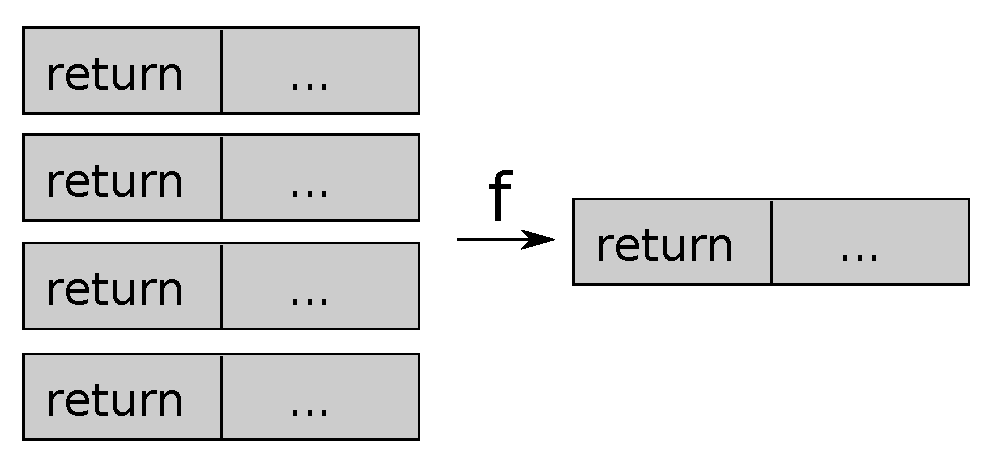
\includegraphics[height=100px]{purity-preservation}

Ist nicht sichergestellt, dass sämtliche Elemente der Eingabeliste rein sind, kann man sich weiter überlegen, dass eine
Möglichkeit zur Verfügung steht, mit der man den reinen Inhalt des monadischen Werts extrahieren kann - ähnlich wie
die unsichere Funktion \texttt{unsafePerformIO}, die den reinen Wert aus einer IO-Monade extrahiert, nur eben für
andere Monaden und sicher.
Es ist ja vorstellbar, dass man nur am reinen Ergebnis einer Funktion $f$ interessiert ist, unabhängig von eventuellen anhaftenden
monadischen Effekten. Tatsächlich kann man unter bestimmten Voraussetzungen zeigen, dass man beliebige Effekte in der 
Eingabeliste ignorieren kann, wenn man nur am reinen Ergebnis interessiert ist.

Sei $f :: Monad\ m \Rightarrow [m\ Int] \rightarrow m\ Int$, sei $\kappa$ eine Monadeninstanz und sei $p :: \kappa\ a \rightarrow a$, d.h. $p$ ist die erwähnte Funktion, die den reinen Wert aus dem monadischen Kontext extrahiert.
Wenn folgende Aussagen gelten:

\begin{itemize}
\item $p \circ return_{\kappa} = id$
\item Für beliebige Typen $t, t'$ und beliebige $m :: k\ t, k :: t \rightarrow k t'$ gilt\\
$p (m\ {>>=}_{\kappa}\ k) = p\ (k\ (p\ m))$
\end{itemize}

dann liefert $p \circ f_{\kappa}$ das gleiche Eregbnis für beliebige Listen gleicher Länge, deren Elemente an jeweils gleicher Position
die gleichen p-Bilder haben, sprich: den gleichen reinen Anteil. Man kann $p \circ f_{\kappa}$ kann also auch erhalten durch
$g \circ (map\ p)$ für eine passende Funktion $g :: [Int] \rightarrow Int$ \cite{voigtlander}.

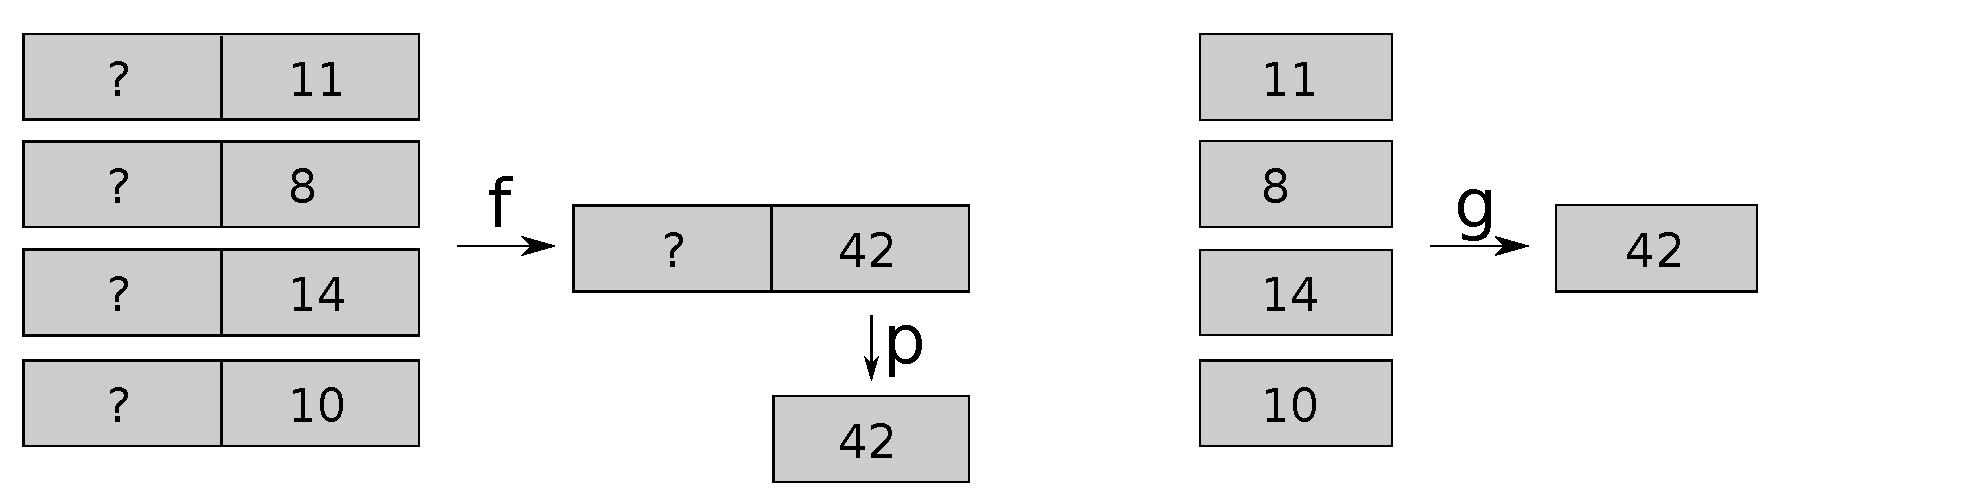
\includegraphics[height=100px]{safe-value-extraction}

Für diese Aussage werden keine Monadengesetze benötigt.

% % % % % % % % % % % % % % % % % % % % % % % % % % % % % % % % % % % % % % % % %
\section{Die Bibliothek free-theorems}
% % % % % % % % % % % % % % % % % % % % % % % % % % % % % % % % % % % % % % % % %

Die Generierung freier Theoreme ist geradlinig und unkompliziert. Gerade deshalb ist es jedoch mühselig, diese Arbeit jedes
Mal per Hand durchzuführen, da ja immer die gleichen Schritte durchgeführt werden. Von daher ist es wünschenswert, diesen
Prozess zu automatisieren, und genau das macht die Bibliothek \textit{free-theorems} \cite{freetheorems}. Diese Bibliothek
beinhaltet die Werkzeuge, die nötig sind, um freie Theoreme aus Haskell-Programmcode zu generieren.

In diesem Kapitel wird näher darauf eingegangen, welche Werkzeuge dies sind und wie sie zusammenspielen. Es wird erläutert,
welche Schritte notwendig sind, um aus Quellcode eine Formel herzuleiten, die das entsprechende freie Theorem beinhaltet.
Abgeschlossen wird diese Übersicht dann mit einem kleinen Beispiel.

%In \cite{freetheorems} wird eine Implementierung vorgestellt, die die automatisierte Generierung von freien Theoremen aus
%Haskell-Code ermöglicht und die Grundlage darstellt, auf die die vorliegende Arbeit aufbaut.
%Sie erlaubt das Parsen von Haskell-Code, das Herausfiltern der entsprechenden Definitionen und deren relationale
%Interpretation, um schließlich die freien Theoreme zu erzeugen.
%Beigefügte Pretty printing Funktionen für Haskell-Syntax und Theoreme vereinfachen schließlich deren Darstellung.

%Im folgenden Abschnitt wird erläutert, wie diese Bibliothek grundlegend aufgebaut ist, wobei auf jeden einzelnen Schritt genauer
%eingegangen wird.


% - - - - - - - - - - - - - - - - - - - - - - - - - - - - - - - - - - - - - - - - - - - - - - - - - - - - - - - - - - - - - - - - - - - - - - - - - - - - - -
\subsection{Aufbau}
% - - - - - - - - - - - - - - - - - - - - - - - - - - - - - - - - - - - - - - - - - - - - - - - - - - - - - - - - - - - - - - - - - - - - - - - - - - - - - -

Die Bibliothek lässt sich grundsätzlich in drei Teile untergliedern: Frontend, Core und Pretty Printer \cite{freetheorems}. Die
Teile werden in dieser Reihenfolge durchlaufen \todo{vgl abbildung}.

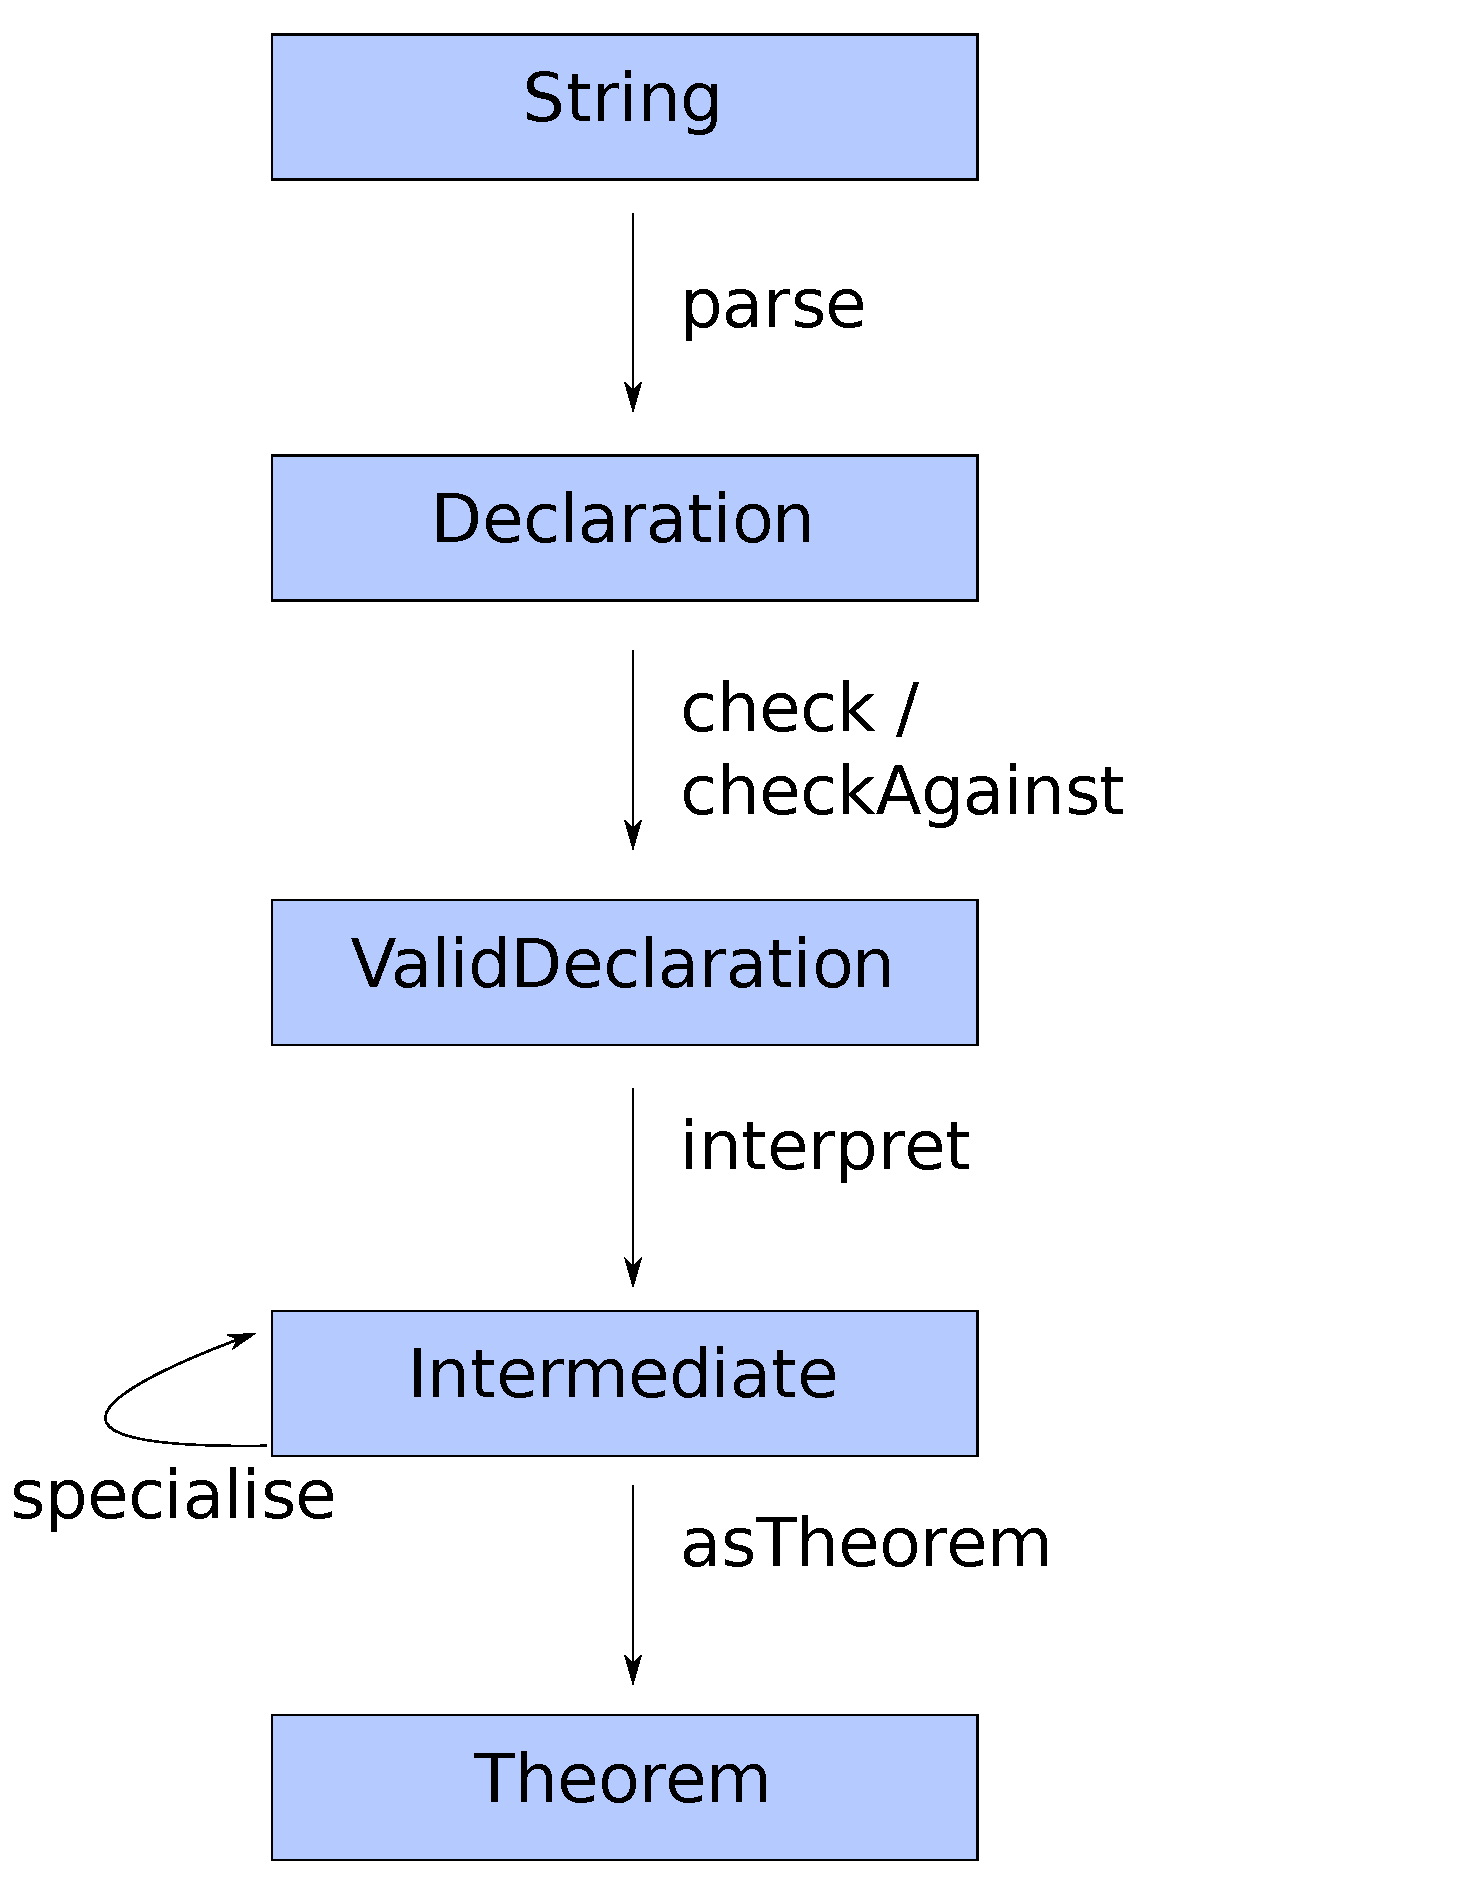
\includegraphics[height=300px]{overview-free-theorems}

Das Frontend ist der Teil, der den Haskell-Code entgegennimmt. Hier wird zunächst der Programmcode geparst und in einen
abstrakten Syntaxbaum übersetzt. Außerdem ist das Frontend dafür zuständig, Fehlerprüfungen durchzuführen und
ungültige Definitionen herauszufiltern, bevor der Syntaxbaum dann weiter an den Core gegeben wird.

%Zunächst werden im Frontend Parser bereitgestellt, um den Haskellcode aus einer Zeichenkette in eine passende Syntaxbaumstruktur umzuwandeln. Mithilfe einer check-Funktion
%wird diese Datenstruktur auf Gültigkeit überprüft, insbesondere in Bezug auf spezielle Anforderungen, die an die Definitionen gestellt wird, um Theoreme zu generieren.

Im Core findet dann die eigentliche Arbeit statt: Hier wird der Syntaxbaum in die entsprechende Relationaldarstellung
überführt und in eine Zwischendarstellung abgelegt, \texttt{Intermediate} genannt. Im nächsten Schritt wird diese
Relationaldarstellung dann Schritt für Schritt abgerollt und in eine Formel überführt. Diese Formel wird schließlich zurückgegeben.

Um diese Formel darzustellen, werden dann im Pretty Printer Teil entsprechende Funktionen bereitgestellt, die in der Lage
sind, den Formel-Datentypen in Zeichenketten umzuwandeln.

%\texttt{interpret} ist dann schließlich die Funktion, die eine Signatur in Bezug auf die anderen Deklarationen in eine Zwischendarstellung \texttt{Intermediate} überträgt. Die
%Funktion \texttt{asTheorem} entfaltet diese Darstellung \todo{``entfaltet''?} schließlich und überträgt sie in den Datentyp \texttt{Theorem}.


% - - - - - - - - - - - - - - - - - - - - - - - - - - - - - - - - - - - - - - - - - - - - - - - - - - - - - - - - - - - - - - - - - - - - - - - - - - - - - -
\subsection{Parser}
% - - - - - - - - - - - - - - - - - - - - - - - - - - - - - - - - - - - - - - - - - - - - - - - - - - - - - - - - - - - - - - - - - - - - - - - - - - - - - -

Um zu einer in Haskell geschriebenen Funktionssignatur irgendetwas zu generieren, muss zunächst eins getan werden: Aus dem
Programmcode muss die notwendige Information herausgezogen werden, der Haskell-Code muss geparst werden.
\textit{free-theorems} erfindet hier das Rad nicht neu sondern setzt auf einen Haskell-Parser, der mit \texttt{haskell-src-exts}
bereits als Paket verfügbar ist \cite{haskellsrcexts} \todo{cite} (bzw. \texttt{haskell-src} als Version, die keine
Spracherweiterungen unterstützt).

Dieses Paket bietet einen Parser für den kompletten Sprachumfang von Haskell inklusive aller Spracherweiterungen, die GHC
unterstüzt \cite{xyz} \todo{cite}. Der Parser liefert eine eigene Datenstruktur für einen abstrakten Syntaxbaum, aber der
enorme Sprachumfang hat natürlich zur Folge, dass dieser Syntaxbaum sehr komplex werden kann. Nun werden aber gar nicht
sämtliche syntaktischen Möglichkeiten der Sprache benötigt, ganz im Gegenteil: Für die Generierung freier Theoreme spielen
hauptsächlich Typsignaturen eine Rolle. Die Implementierungen, die in einem typischen Programm den Großteil des Programms
ausmachen, können getrost vernachlässigt werden.

Aus diesem Grund führt \textit{free-theorems} eine eigene Syntaxbaum-Datenstruktur ein und überführt den Syntaxbaum,
der von \texttt{haskell-src-exts} generiert wird, in eine vereinfachte Darstellung, genannt \texttt{BasicSyntax}.

%Neben dem Haskell 98 Parser, der keine \todo{Keine?} Spracherweiterungen zulässt, ist auch der Hsx Compiler gegeben, der die
%komplette Sprache mitsamt Spracherweiterungen umsetzt. Hier ist anzumerken, dass das Paket free-theorems in seiner aktuellen Form
%nicht mit dem aktuellen Haskell-Compiler kompatibel war und einige Anpassungen gemacht werden mussten. \todo{Evtl im Anhang Näheres?}
%Intern nutzt free-theorems hier die Pakete \texttt{Language.Haskell.Parser} bzw. \texttt{Language.Haskell.Exts.Parser}, die an sich bereits voll funktionstüchtige Parser liefern.

%Allerdings ist der komplette Sprachumfang sehr komplex und ein Arbeiten mit den Datenstrukturen, die von diesen genutzten Parsern generiert werden,
%wird unnötig erschwert. Aus diesem Grund transformiert free-theorems diese Datenstruktur in eine eigene, vereinfachte Struktur namens BasicSyntax. In dieser Struktur
%werden lediglich Typsignaturen festgehalten, Implementierungen werden vollkommen ignoriert, da sie für die Theoremgenerierung keine Rolle spielen.


\subsubsection{BasicSyntax}
% `````````````````````

Ein paar kleine Beispiele sollen ein Gefühl dafür vermitteln, wie der \texttt{BasicSyntax}-Datentyp aussieht. Dabei ist jeweils
eine Funktionssignatur gegeben und dahinter die Haskell-Darstellung des resultierenden BasicSyntax-Ausdrucks.

\begin{listing}[ht]
\inputminted[tabsize=2]{haskell}{ast.hs}
\caption{Beispiel}
\label{lst:ast}
\end{listing}

Listing \ref{lst:ast} zeigt die Datenstruktur am Beispiel \texttt{test :: [a] $\rightarrow$ [a]}. Die \texttt{parse}-Funktion des Parser-Moduls von \textit{free-theorems} liefert eine Liste sämtlicher relevanter Definitionen als \texttt{BasicSyntax} zurück.
In diesem Beispiel ist nur eine Typsignatur gegeben, \texttt{parse} gibt also eine einelementige Liste zurück, bestehend aus
genau einem Konstruktor \texttt{TypeSig}.

Da man freie Theoreme aus den Typsignaturen von Funktionen herleitet, könnte man sich überlegen, dass man auf alles andere
als Typsignaturen verzichten kann und der Rest des Programms irrelevant ist. Während dies für Implementierungen der Funktionen,
also die jeweiligen Funktionsrümpfe, zutrifft, gibt es dennoch andere Deklarationen, an denen man ebenfalls interessiert ist.

Man bekommt nämlich genau dann ein Problem, wenn der Entwickler im Programm eigene Datentypen deklariert und diese in
den Funktionssignaturen verwendet. Neben Funktionssignaturen werden also zusätzlich auch Datentypdeklarationen benötigt.
Hierzu gehören sowohl die \texttt{data}- als auch \texttt{type}- und \texttt{newtype}-Deklarationen (die semantischen Unterschiede
zwischen diesen verschiedenen Deklarationen spielen dabei keine Rolle). Listing \ref{lst:ast-data} zeigt ein Beispiel für eine
\texttt{data}-Deklaration und deren entsprechende Darstellung als \texttt{BasicSyntax}.

An diesem Beispiel kann man ebenfalls sehen, dass die Konstruktorparameter in die \texttt{Unbanged}-Struktur eingebettet sind.
Es gibt \texttt{Unbanged} und \texttt{Banged}, was einfach sagt, ob eine Striktheitsannotation vor dem entsprechenden
Parameter steht oder nicht. Es soll hier nicht näher darauf eingegangen werden, wozu diese Annotation verwendet wird, in
Kapitel \ref{sec:striktheit-und-rekursion} wird noch ein bisschen näher darauf eingegangen.

Klassendeklarationen werden insbesondere in Kapitel \ref{sec:erweiterung-um-typklassen} benötigt. Sie werden aber auch schon
von \texttt{free-theorems} beachtet und in die \texttt{BasicSyntax} mit aufgenommen. Der Grund dafür ist der, dass ja auch
Typvariablen in Typsignaturen auftreten können, die auf eine bestimmte Klasse eingeschränkt sind. Die aus der Allquantifizierung
resultierenden Relationen dürfen also nicht über alle Typen quantifiziert sein, sondern nur über solche, die zur entsprechenden
Klasse passen.

%Natürlich ist man hauptsächlich an den Funktionssignaturen interessiert, da man aus diesen die Theoreme ableitet. Aber natürlich können diese Signaturen ihrerseits wiederum 
%selbst definierte Datentypen oder auch Klasseneinschränkungen enthalten. Man kommt also nicht umhin, auch diese mit einzubeziehen und ebenfalls in der BasicSyntax vorzusehen.
%Das Beispiel in Listing \ref{lst:ast-data} zeigt eine data-Deklaration.

\begin{listing}[ht]
\inputminted[tabsize=2]{haskell}{ast2.hs}
\caption{Beispiel}
\label{lst:ast-data}
\end{listing}


% - - - - - - - - - - - - - - - - - - - - - - - - - - - - - - - - - - - - - - - - - - - - - - - - - - - - - - - - - - - - - - - - - - - - - - - - - - - - - -
\subsection{check}
% - - - - - - - - - - - - - - - - - - - - - - - - - - - - - - - - - - - - - - - - - - - - - - - - - - - - - - - - - - - - - - - - - - - - - - - - - - - - - -

\label{sec:check}

An dieser Stelle liegt das Eingabeprogramm also in einem vereinfachten abstrakten Syntaxbaum vor. Da der Parser das Programm
erfolgreich geparst hat, können Parserfehler ab hier ausgeschlossen werden. Der Haskell-Parser ist aber wirklich nur dazu da,
Haskell-Code in einen Syntaxbaum zu überführen, über Syntax hinausgehende Fehler werden nicht erkannt. Aus diesem Grund
muss der Syntaxbaum jetzt auf semantische Fehler überprüft werden, was in der \texttt{check}-Funktion geschieht.

Fehlerhafte Deklarationen werden aus der Liste der Deklarationen gefiltert, und es werden entsprechende Fehlermeldungen
generiert. Fehler führen hier nicht automatisch zum Abbruch, es ist ja durchaus möglich, dass die Fehler in Deklarationen
auftreten, die für die betrachtete Funktionssignatur keine Rolle spielen.

Es wird zwischen lokaler und globaler Fehlerprüfung unterschieden. Lokale Prüfungen werden pro Deklaration durchgeführt,
ohne den globalen Kontext zu betrachten. Hier werden lediglich solche Fehler betrachtet, die sich anhand der Deklaration selbst
erkennen lassen. Ein Beispiel sind \texttt{data}-Deklarationen: Hier müssen auf der rechten Seite auftretende Typvariablen
auch auf der linken Seite vorkommen; einen Fehler würde beispielsweise folgender Code erzeugen.

\begin{minted}{haskell}
data Test = Test a
\end{minted}

Außerdem müssen alle Variablennamen auf der linken Seite paarweise verschieden sein, primitive Datentypen dürfen nicht
neu deklariert werden, usw.

Nach den lokalen Überprüfungen finden die globalen Checks statt. Hier geht es um solche Prüfungen, bei denen stets das komplette
Programm betrachtet werden muss, zum Beispiel um sicherzustellen, dass alle Funktionsnamen im Programm deklariert sind,
pro Funktionsname nur eine Deklaration existiert, Typkonstruktoren die korrekte Anzahl an Parametern haben etc.

Eine besondere Aufgabe der globalen Überprüfung ist es auch, sämtliche Typausdrücke zu \textit{schließen}; es ist in Haskell
erlaubt, freie Typvariablen in Funktionssignaturen zu verwenden - diese werden implizit als allquantifiziert angesehen.
Das Schließen eines Typausdrucks besteht nun darin, sämtliche freien Typvariablen zu beseitigen, indem eine entsprechende
explizite Allquantifizierung davorgesetzt wird.

So kann im weiteren Programmverlauf davon ausgegangen werden, dass keine freien Typvariablen mehr vorkommen, was die
Verarbeitung erleichtert.
%Dabei wird dafür gesorgt, dass keine freien Typvariablen mehr in Typsignaturen vorkommen, indem die entsprechenden Variablen durch einen


% % %

%Im zweiten Schritt wird die \texttt{check}-Funktion benutzt, um alle Deklarationen auf Gültigkeit zu überprüfen und die Liste der Deklaration zu filtern. Ungültige Deklarationen
%werden unter Angabe einer Fehlermeldung aus der Liste entfernt \cite{freetheorems}.
%
%Es ist zwar davon auszugehen, dass die Syntax des Programmes korrekt ist, da ansonsten der Haskell-Parser bereits im ersten Schritt einen Fehler gemeldet hätte, dennoch ist
%dieser zweite Schritt nötig, um auch korrekte Semantik voraussetzen zu können \todo{wahrscheinlich falsch ausgedrückt} (da andernfalls auch für fehlerhafte Programme Theoreme generiert würden, was keinen Sinn macht).
%
%Die check-Funktion untergliedert sich in lokale und globale Checks, wobei die lokalen Checks pro Definition durchgeführt werden, die globalen Checks beziehen sich auf die Gesamtheit aller Definitionen. Beispielsweise wird lokal überprüft, ob bei Deklarationen die freien Variablen auf der rechten Seite auf der linken Seite der Defintion deklariert sind, es wird sichergestellt
%dass auf der linken Seite alle Variablennamen verschieden sind, primitive Datentypen nicht deklariert werden usw.
%
%Unter die globalen Checks fällt z.B., dass zu einem Funktionsnamen nicht mehrere Deklarationen existieren, dass alle Typkonstruktoren die korrekte Anzahl an Parametern haben oder auch dass keine Kreise in der Typklassenhierarchie existieren \cite{freetheorems}.
%
%Am Ende schließt \texttt{check} noch alle Typausdrücke, dh. bei frei vorkommenden Typvariablen werden entsprechende Typabstraktionen um den Ausdruck geschlossen. Das ist wichtig, da in der weiteren Implementierung davon ausgegangen wird, dass alle Typausdrücke geschlossen sind und entsprechende Typabstraktionen zu jeder implizit allquantifizierten Variable vorhanden sind.

Tabelle \ref{tab:global-checks} zeigt eine Übersicht aller globalen Überprüfungen.

\begin{table}[th]
\centering
\begin{tabular}{| l | l |}
\hline
Name&Prüfung\\
\hline
  checkUnique&Alle Namen kommen nur einmal vor\\
  checkArities&Typkonstruktoren haben korrekte Anzahl an Parametern\\
  checkAcyclicTypeSynonyms&Typsynonyme sind azyklisch\\
  checkAcyclicTypeClasses&Typklassen sind azyklisch\\
  checkAllConsAndClassesDeclared&Alle Typkonstruktoren und Typklassen sind deklariert\\
\hline
\end{tabular}
\caption{Globale Überprüfungen}
\label{tab:global-checks}
\end{table}

Sind alle globalen Überprüfungen abgeschlossen, werden die übrig bleibenden Deklarationen an den Core-Teil weitergereicht.


% - - - - - - - - - - - - - - - - - - - - - - - - - - - - - - - - - - - - - - - - - - - - - - - - - - - - - - - - - - - - - - - - - - - - - - - - - - - - - -
\subsection{interpret}
% - - - - - - - - - - - - - - - - - - - - - - - - - - - - - - - - - - - - - - - - - - - - - - - - - - - - - - - - - - - - - - - - - - - - - - - - - - - - - -

\label{sec:free-theorems-interpret}

Die erste Funktion des Cores ist \texttt{interpret}. Diese Funktion \textit{interpretiert} eine Funktionssignatur als Relation. Sie
erwartet eine (geprüfte) Deklaration als Eingabe und liefert eine Relation, verpackt in eine sogenannte \texttt{Intermediate}-Struktur,
die neben der eigentlichen Relation noch Zusatzinformationen beinhaltet, beispielsweise den Namen der interpretierten Funktion
sowie freie Variablennamen für neu einzuführende Variablen.
Diese Funktion setzt also den Schritt um, die Funktionssignatur in die Relationsschreibweise zu überführen.

\texttt{interpret} durchläuft rekursiv die \texttt{BasicSyntax}-Struktur und erzeugt entsprechende Relationen.
Tabelle \ref{tab:relations} zeigt, welche Konstruktoren der \texttt{Relation}-Datentyp hat. Dabei ist zu beachten, dass
\texttt{FunVar} nur verwendet wird, wenn Relationen zu Funktionen spezialisiert werden. \todo{referenz auf spaeter}

\begin{table}
\centering
\begin{tabular}{| l | l | l |}
\hline
BasicSyntax & Relation & Mathematische Entsprechung\\
\hline
TypeVar & RelVar & $\alpha$ \\
FunVar & - & f \\
TypeCon & RelBasic & $\mathcal{R}$ \\
& RelLift & [$\mathcal{R}$], etc. \\
TypeFun & RelFun & $S \rightarrow T$ \\
& RelFunLab & $S \rightarrow T$ \\
TypeAbs & RelAbs & $\forall R . F R$ \\
& FunAbs &\\
\hline
\end{tabular}
\caption{Konstruktoren des Datentyps Relation}
\label{tab:relations}
\end{table}

Wie vorangehend erwähnt, werden sämtliche freie Variablen in Typsignaturen eliminiert, was dazu führt, dass \texttt{interpret}
stets zuerst auf einen \texttt{forall}-Ausdruck stoßen wird, bevor es die Typvariable selbst antrifft. Das wird ausgenutzt, indem
beim Antreffen von \texttt{forall} ein Eintrag in einer Map angelegt wird, auf den dann bei Verarbeitung jedes Vorkommens der
Typvariable über den Variablennamen wieder zugegriffen wird.

Ansonsten wird systematisch jeder Ausdruck der \texttt{BasicSyntax} durch den entsprechenden \texttt{Relation}-Ausdruck
ersetzt. Typkonstruktorausdrücke werden entweder zu einer \texttt{RelBasic}, also einer einfachen Relation auf Typmengen,
oder zu \texttt{RelLift}-Ausdrücken, also \textit{gelifteten} Relationen, je nachdem ob es sich um nullstellige oder mehrstellige
Typkonstruktoren handelt.

Aus der Funktion resultiert also letztendlich ein \texttt{Relation}-Ausdruck, der im nächsten Schritt weiterverarbeitet wird.

% % %

%Tatsächlich macht die \texttt{interpret}-Funktion nichts, was nicht schon bekannt ist \todo{Das heißt, wenn ich es denn schon geschrieben hätte}: Sie überführt die Funktionssignatur in eine
%Relationsdarstellung, wobei sie Typvariablen neu generierte Relationsvariablen zuordnet. Um es mit der Aufteilung von \cite{freetheorems} auszudrücken, stellt sie den Übergang des Frontends zum Core dar, wo der interessante Arbeitsschritt ausgeführt wird.

%Der Datentyp, der hier verwendet wird, heißt Immediate. Dieser Datentyp ist letztlich nur ein Container für eine Relation mit
%dem repräsentierten Typausdruck, zusätzlichen (unendlichen) Listen von freien Variablennamen und sonstigen Zusatzinformationen.

%
%\subsubsection{Relation}
%% ``````````````````
%
%Für die Darstellung als Relationen definiert free-theorems den Datentyp \texttt{Relation}, der folgende Konstruktoren hat:
%
%\todo{unvollständig. und evtl unnötig}
%
%Wie man sieht, fehlt noch ein Konstruktor für die neu eingeführte Variante, dass eine Typkonstruktorvariable auf Relationen
%angewandt wird. Darauf wird in Abschnitt \ref{sec:erweiterung-typklassen} eingegangen.


% - - - - - - - - - - - - - - - - - - - - - - - - - - - - - - - - - - - - - - - - - - - - - - - - - - - - - - - - - - - - - - - - - - - - - - - - - - - - - -
\subsection{Spezialisieren von Relationsvariablen zu Funktionen}
% - - - - - - - - - - - - - - - - - - - - - - - - - - - - - - - - - - - - - - - - - - - - - - - - - - - - - - - - - - - - - - - - - - - - - - - - - - - - - -

\label{sec:specialise-relvars}

Der Spezialisierungsschritt ist optional. Wie in den Grundlagen erläutert, kann man jede Funktion auch als Relation auffassen,
Funktionen sind also spezielle Relationen. Hat man eine allgemeine Aussage über beliebige Relationen, dann trifft dieselbe
Aussage auch auf alle solche Relationen zu, bei denen es sich um Funktionen handelt - man spezialisiert die Aussage einfach
auf Funktionen.

Es bietet sich an, das zu tun, weil die Funktionsdarstellung übersichtlicher und intuitiver verständlich ist. Aus diesem Grund
bietet \textit{free-theorems} die Funktion \texttt{specialise} an. Diese Funktion erwartet eine Intermediate-Struktur und
eine Relationsvariable und transformiert die Intermediate-Struktur, indem sie sämtliche vorkommen der Relationsvariablen
durch Funktionsvariablen ersetzt.

Im zweiten Schritt führt sie die \texttt{reduceLifts}-Funktion aus, die versucht geliftete Datentypen zu vereinfachen.
\todo{besser ausdrücken} Wenn es sich hierbei um eine Funktion handelt, dann wird überprüft, ob es sich beim Typen
um Listen oder um den spezifischen Typen \texttt{Maybe} handelt. In diesen Fällen wird der Ausdruck ersetzt durch die
Funktion $map$ bzw. $fmap$, angewandt auf die entsprechende Funktion. Man kann dies als das \textit{Lifting} der Funktion
in den entsprechenden Kontext auffassen.

Am einfachsten lässt sich das an einem Beispiel zeigen.

\begin{minted}{haskell}
test :: a -> [a]
\end{minted}

Man kann leicht nachvollziehen, dass diese Signatur zu folgendem freien Theorem führt.

\begin{align*}
& \forall T_1, T_2 \in Types, \mathcal{R} : T_1 \Leftrightarrow T_2 \\
& \forall (x, y) \in \mathcal{R} \\
& (test_{T1}\ x, test_{T2}\ y) \in lift_{[]}(\mathcal{R})
\end{align*}

Ersetzt man die Relationsvariablen jetzt durch Funktionensvariablen, ergibt sich die folgende Aussage.

\begin{align*}
& \forall f : T_1 \rightarrow T_2 \\
& \forall x \in T_1 \\
& lift_{[]}(f) (test_{T_1}\ x) = test_{T2} (f\ x)
\end{align*}

Zu beachten ist hier, dass der letzte Schritt nicht zwingend durchgeführt werden kann. Ein solches Lifting ist nur in besonderen
Fällen möglich, in diesem Fall entspricht das Lifting der Funktion $f$ in den Listenkontext ganz einfach der Haskell-Funktion
\texttt{map}. Das Theorem lässt sich also auch wie folgt ausdrücken.

\begin{align*}
& \forall f : T_1 \rightarrow T_2 \\
& \forall x \in T_1 \\
& map\ f\ (test_{T_1}\ x) = test_{T2} (f\ x)
\end{align*}

Handelt es sich um den Typen \texttt{Maybe}, lässt sich stattdessen $fmap\ f$ verwenden.

Die \texttt{asTheorem}-Funktion, die im nächsten Abschnitt erläutert wird, arbeitet sowohl mit Relationsvariablen als auch mit
Funktionsvariablen.
%Ist das Theorem generiert, kann man nun die Funktionsrelation spezialisieren, um das Theorem zu vereinfachen. Aus einem
%$A : S \leftrightarrow T$ wird also $\forall a : S \rightarrow T$

%usw.


% - - - - - - - - - - - - - - - - - - - - - - - - - - - - - - - - - - - - - - - - - - - - - - - - - - - - - - - - - - - - - - - - - - - - - - - - - - - - - -
\subsection{asTheorem}
% - - - - - - - - - - - - - - - - - - - - - - - - - - - - - - - - - - - - - - - - - - - - - - - - - - - - - - - - - - - - - - - - - - - - - - - - - - - - - -

Der Schritt, der zu Beginn als ``Abrollen'' der Parametrizitätsaussage eingeführt wurde, wird in der Funktion \texttt{asTheorem}
durchgeführt. Wie in Abschnitt \ref{sec:free-theorems-param} erläutert, gilt zu jeder aus einer Typsignatur hergeleiteten
Relation das Parametrizitäts-Theorem der Form $(e, e) \in \mathcal{R}$ ($e$ ist der Ausdruck, $\mathcal{R}$ ist die hergeleitete
Relation).

Als Eingabe erwartet \texttt{asTheorem} sinnigerweise die Intermediate-Struktur aus den vorangegangenen Schritten. Diese wird
nun rekursiv in eine Formel umgewandelt. Als Ergebnis liefert die Funktion eine \texttt{Formula}, wobei es sich um einen
Datentyp handelt, der die Darstellung von Formeln ermöglicht. Man kann diesen Datentyp als eine Vorstufe zur reinen
Zeichenkette ansehen, denn er stellt in keinster Weise sicher, dass die Formeln sinnvoll sind. Lediglich syntaktische Korrektheit
ist durch Verwenden der Datenstruktur gegeben.

%Grundsätzlich nutzt \texttt{asTheorem} eine Reihe von \texttt{unfold}-Funktionen, die jeweils einen Konstruktor des
%Relation-Datentyps abdecken. Die oberste Funktion ist \texttt{unfoldFormula}, die die folgende Signatur hat.

Intern ruft die Funktion eine Funktion namens \texttt{unfoldFormula} auf, die die folgende Signatur hat.

\begin{minted}{haskell}
unfoldFormula :: Term -> Term -> Relation -> Unfolded Formula
\end{minted}

Die Parameter entsprechen dabei dem Ausgangsausdruck $(x, y) \in \mathcal{R}$, wobei $\mathcal{R}$ eine (eventuell aus
Relationen konstruierte) Relation ist, deren Definition angewandt werden soll. Handelt es sich bei $\mathcal{R}$ beispielsweise
um eine einfache Relationsvariable, gibt \texttt{unfoldFormula} die Formel $(x, y) \in \mathcal{R}$ zurück. Handelt es sich
um eine \texttt{RelBasic}, d.h. sie ist aus einem nullstelligen Typkonstruktor entstanden (z.B. \texttt{Int}), dann wird hingegen
die Formel $x = y$ zurückgegeben, da in der Basistypen durch Identitätsrelationen dargestellt werden und $x$ und $y$ folglich
nur verwandt sein können, wenn sie gleich sind.

Hinter dem Rückgabewert \texttt{Unfolded Formula} verbirgt sich noch eine Monade, mit der eventuell auftretende Fehlermeldungen
durchgereicht werden können. Das interessante Ergebnis ist die resultierende Formel, die als \texttt{Formula} zurückgegeben wird.

Konkret bedeutet das also: Wird die Funktion \texttt{asTheorem} mit einer Intermediate-Struktur aufgerufen, die den
Funktionsnamen \texttt{n} und die Relation \texttt{r} beinhaltet, wertet sie den folgenden Ausdruck aus.

\begin{minted}{haskell}
unfoldFormula n n r
\end{minted}

% TODO: noch weiter ins detail gehen?

%Die \texttt{asTheorem}-Funktion stellt eine Datenstruktur des Typs \texttt{Intermediate} als Theorem dar. Tatsächlich passiert hier aber eine ganze Menge mehr als der Name
%vermitteln mag. Das schrittweise Abrollen der Relationen stellt schließlich den entscheidenden Schritt dar, durch den man überhaupt auf
%die Theoreme schließen kann.
%
%\todo{Hier eventuell auch ein Beispiel?}


% - - - - - - - - - - - - - - - - - - - - - - - - - - - - - - - - - - - - - - - - - - - - - - - - - - - - - - - - - - - - - - - - - - - - - - - - - - - - - -
\subsection{simplify}
% - - - - - - - - - - - - - - - - - - - - - - - - - - - - - - - - - - - - - - - - - - - - - - - - - - - - - - - - - - - - - - - - - - - - - - - - - - - - - -

An dieser Stelle liegt die Formel im \texttt{Formula}-Datentyp vor. Bevor sie schließlich mithilfe der Pretty Printer Funktionen
in eine Zeichenkette umgewandelt wird, kann optional noch die \texttt{simplify}-Funktion aufgerufen werden, die einige
Vereinfachungen auf die Formel anwendet. Diese Funktion hat keine Kenntnis von der ursprünglichen Relationaldarstellung, sie
vereinfacht einfach nur typische Muster.

Ein Beispiel wäre zum Beispiel das Entfernen aller unbenutztzen allquantifizierten Variablen, wie in der folgenden Formel zu sehen
ist.

\begin{align*}
& \forall v \forall x . x = x \\
\Leftrightarrow & \forall x . x = x 
\end{align*}

Auch möglich ist zum Beispiel die folgende Vereinfachung, die im Zusammenhang mit freien Theoremen häufig angewandt werden
kann.

\begin{align*}
&\forall v . f\ v = g\ v\\
\Leftrightarrow & f = g
\end{align*}

Die Funktion \texttt{simplify} erwartet also eine \texttt{Formula} und transformiert diese. Die resultierende Formel kann
dann per Pretty Printer in eine Zeichenkette umgewandelt werden.

%Schließlich bietet free-theorems noch die Möglichkeit, die generierten Theoreme zu vereinfachen, indem nach einigen typischen
%Mustern gesucht wird, beispielsweise: Entfernen aller unbenutzten allquantifizierten Variablen, $\forall v. f v == g v \rightarrow f == g$ usw.


% - - - - - - - - - - - - - - - - - - - - - - - - - - - - - - - - - - - - - - - - - - - - - - - - - - - - - - - - - - - - - - - - - - - - - - - - - - - - - -
\subsection{unfoldLifts, unfoldClasses}
% - - - - - - - - - - - - - - - - - - - - - - - - - - - - - - - - - - - - - - - - - - - - - - - - - - - - - - - - - - - - - - - - - - - - - - - - - - - - - -

Schließlich bietet \textit{free-theorems} noch die Möglichkeit, die verwendeten Datentypen und Typklassen aus einer
Signatur zu extrahieren und jeweils eine Relationaldarstellung zu generieren. Wie in Abschnitt \ref{sec:free-theorems-param}
bereits beschrieben, stellt man verwendete Datentypen, die eine freie Typvariable als Parameter erwarten, als Relationen
dar. Das Vorgehen ist auch hier sehr generisch, sodass dies von einer Funktion übernommen werden kann. Betrachten wir
das folgende Beispiel.

\begin{minted}{haskell}
data MyType a = MyCons String Int a | MyOtherCons String

test :: MyType a -> a
\end{minted}

In der Funktionssignatur zu \texttt{test} findet der selbstdefinierte Datentyp \texttt{MyType} Verwendung. Ihm wird die
Typvariable \texttt{a} als Parameter übergeben. Im freien Theorem wurde die relationale Repräsentation eines gelifteten
Datentyps immer durch eine Funktion \textit{lift} dargestellt. \textit{free-theorems} bietet die Funktion \texttt{unfoldLifts},
die sämtliche Lifts aus dem Theorem extrahiert und deren Definition als Formel generiert.

Auch bei benutzerdefinierten Datentypen geht es letztlich darum, welche Ausdrücke \textit{verwandt} sind bezüglich der
Relation. Ein Datentyp hat stets verschiedene Konstruktoren. In der Relation entspricht das der Vereinigung verschiedener
Teilmengen, eine Teilmenge pro Konstruktor. Die folgende Formel ergibt sich aus dem obigen Beispiel.

\begin{minted}{haskell}
"lift{MyType}(R)
  = {(MyCons x1 x2 x3, MyCons y1 y2 y3) |
       ((x1 = y1) && (x2 = y2)) && ((x3, y3) in R)}
  u {(MyOtherCons x1, MyOtherCons y1) | x1 = y1}"
\end{minted}

Es wird einfach das bekannte Prinzip weitergeführt: Ausdrücke von Basistypen sind verwandt, wenn sie gleich sind. Ausdrücke
des polymorphen Typen, der als Typvariable übergeben wurde, sind genau dann verwandt, wenn sie in der zugrundeliegenden
Relation verwandt sind.

Eine weitere Funktion, die \textit{free-theorems} anbietet, ist \texttt{unfoldClasses}. Diese Funktion extrahiert die Klassen,
die im Theorem eine Rolle spielen, und erstellt zu jeder Klasse eine Formel, die beschreibt, wann Relationen diese Klasse
\textit{respektieren}. Dabei wird die entsprechende Formel automatisch abgerollt. Im Folgenden wird dies an einem Beispiel
verdeutlicht.

\begin{minted}{haskell}
class TestClass t where
   testfun :: t -> t

test :: TestClass t => t -> t
\end{minted}

Für dieses Beispiel erzeugt die Funktion \texttt{unfoldClasses} die folgende Formel.

\begin{minted}{haskell}
"R respects TestClass if
  forall (x, y) in R. (testfun_{t1} x, testfun_{t2} y) in R"
\end{minted}

% - - - - - - - - - - - - - - - - - - - - - - - - - - - - - - - - - - - - - - - - - - - - - - - - - - - - - - - - - - - - - - - - - - - - - - - - - - - - - -
\subsection{Beispiel}
% - - - - - - - - - - - - - - - - - - - - - - - - - - - - - - - - - - - - - - - - - - - - - - - - - - - - - - - - - - - - - - - - - - - - - - - - - - - - - -

In den vorangegangenen Abschnitten wurde ein kurzer Umriss der Bibliothek free-theorems gegeben, die im Folgenden um
Typkonstruktorklassen erweitert werden soll. Bevor die benötigten Änderungen erläutert werden, soll hier zunächst ein
kompletter Durchlauf als Beispiel gegeben werden. Es werden sämtliche Daten betrachtetet, die auf dem Weg von einer
Eingabezeichnekette zur resultierenden Ausgabezeichenkette entstehen.

\todo{Grafik}

Wir bemühen das Beispiel aus dem vorangegangenen Kapitel. Die Typsignatur ist simpel genug,
um die grundlegende Funktionsweise zu erläutern, ohne die auftretenden Datenstrukturen unnötig kompliziert zu machen.

\begin{minted}{haskell}
f :: [a] -> [a]
\end{minted}

Im ersten Schritt setzt man einen bereitgestellten Parser ein, um diesen Haskell-Code in den bibliotheksinternen, vereinfachten
Syntaxbaum \texttt{BasicSyntax} zu parsen. Die \texttt{parse}-Funktion gibt genaugenommen eine Liste von \texttt{Declaration}s, also Deklarationen. Dabei handelt es sich um alle Toplevel-Deklarationen, die eine Rolle spielen, also Funktionssignaturen,
Datentypdeklarationen und Klassendeklarationen.

%[
%   (TypeSig
%      (Signature {
%         signatureName = (Ident {unpackIdent = "test"}),
%         signatureType =
%            (TypeAbs (TV (Ident {unpackIdent = "a"}))
%               []
%               (TypeFun
%                  (TypeVar
%                     (TV (Ident {unpackIdent = "a"}))
%                  )
%                 (TypeVar (TV (Ident {unpackIdent = "a"})))
%               ))}))
%]

\begin{minted}{haskell}
(TypeSig (Signature {
   signatureName = (Ident "test"),
   signatureType =
      (TypeAbs (TV (Ident "a"))
         []
         (TypeFun
            (TypeCon ...
               [(TypeVar (TV (Ident "a")))]
            )
            (TypeCon ...
               [(TypeVar (TV (Ident "a")))]
            )
         )
      )
   })
)
\end{minted}

Hier wurde die Darstellung ein wenig vereinfacht, um das Verständnis zu erleichtern. Zu beachten ist aber, dass sämtliche
Funktionsimplementierungen wegfallen. Sie spielen für die Generierung freier Theoreme keine Rolle, das bedeutet aber auch,
dass free-theorems keine Fehlerprüfungen im Implementierungsteil durchführt. Die Bibliothek kann ohne Auftreten von Fehlern
durchlaufen, selbst der zu einer Funktionssignatur gehörige Code Fehler enthält.

Jetzt, da die \texttt{BasicSyntax} der Beispielfunktion vorhanden ist, muss \texttt{check} aufgerufen werden, um Fehler
zu entdecken. Ein Aufruf macht aus der Liste von \texttt{Declaration}s eine Liste von \texttt{ValidDeclaration}s. Tatsächlich
enthält diese Datenstruktur lediglich ein zusätzliches Feld \texttt{isStrictDeclaration}, das anzeigt, ob die entsprechende
Deklaration strikte Elemente enthält oder von diesen abhängt.

Um genau zu sein, ist der Ergebnistyp von \texttt{check} monadisch, es werden per Writer-Monade Fehlermeldungen
generiert, falls Fehler auftreten. Es ist noch anzumerken, dass \texttt{check} auch beim Auftreten von Fehlern eine Liste
von Deklarationen zurückgibt. Lediglich die Deklarationen, die Fehler enthalten, werden weggelassen; das bedeutet, dass
unter Umständen Theoreme generiert werden können, wenn nur Fehler auftreten, die keine Auswirkung auf das zu generierende
Theorem haben.

\begin{minted}{haskell}
[(ValidDeclaration (TypeSig ...) False)]
\end{minted}

An dieser Stelle haben wir eine Liste gültiger Deklarationen, und wir haben eine Liste eventell aufgetretener Fehler. Um nun
freie Theoreme zu einer Typsignatur zu generieren, wird zunächst einmal eine Typsignatur benötigt. free-theorems bietet die
Funktion \texttt{filterTypeSignatures}, um Typsignaturen aus einer Liste von \texttt{ValidSignature}s herauszufiltern, was in
unserem Beispiel keinen Unterschied macht, weil es lediglich aus einer Typsignatur besteht.

Jetzt können wir \texttt{interpret} verwenden, um zu unserer \texttt{ValidSignature} unter Verwendung der übrigen
\texttt{Declaration}s die Relationaldarstellung unsereres Datentyps zu generieren. Das Ergebnis sieht wie folgt aus.

\begin{minted}{haskell}
(Intermediate "test" BasicSubset
   (RelAbs "R" ("t1", "t2")
      (RelFun
         (RelLift ("[t1]", "[t2]") ConList (RelVar "R"))
         (RelLift ("[t1]", "[t2]") ConList (RelVar "R"))
      )
   )
   ...
)
\end{minted}

Auch dieses Beispiel ist stark vereinfacht dargestellt, beinhaltet aber die wichtigsten Elemente. Zu beachten ist vor allem,
dass es sich bei den Tupeln \texttt{("[t1]'', "[t2]'')} nicht wirklich um Tupel von Zeichenketten handelt, tatsächlich sind dies
\texttt{TypeExpression}s der \texttt{BasicSyntax}-Struktur. Der Einfachheit halber werden diese hier jedoch als Zeichenketten
dargestellt, da ihre tatsächliche Form im Folgenden auch keine wirkliche Rolle mehr spielt.

Wie man sehen kann, wird alles in den \texttt{Intermediate}-Datentyp eingerahmt. Dieser enthält den Namen des Ausdrucks, d.h.
den Funktionsnamen, für den die Typsignatur überhaupt angegeben wird. Zudem ist angegeben, welche \textit{Sublanguage}
verwendet wird. In diesem Fall ist dies \texttt{BasicSubset}; dieser Wert hängt davon ab, wie \texttt{interpret} aufgerufen wurde.

Ansonsten spiegelt die Struktur ziemlich genau den Aufbau der \texttt{TypeSig}-Struktur wider. Zur Erinnerung: An dieser Stelle
wird die Typsignatur auch lediglich als Konstruktion aus verschiedenen Relationaldarstellungen zusammengesetzt. Wie diese
im Einzelnen definiert sind, spielt hier noch keine Rolle.

Nun soll der Ausdruck auf Funktionen spezialisiert werden. In den bisherigen Beispielen wurde die Aussage zunächst abgerollt, dann
wurde ganz am Ende die Aussage spezialisiert. Es spielt für die Korrektheit der Aussage keine Rolle, ob sie zuerst abgerollt wird, oder ob
zuerst Relationsvariablen auf Funktionsvariablen spezialisiert werden und das Abrollen danach stattfindet.

Es wird also die Funktion \texttt{specialise} aufgerufen, die den Ausdruck folgendermaßen transformiert.

\begin{minted}{haskell}
(Intermediate "test" BasicSubset 
   (FunAbs "f" ("t1", "t2")
      (RelFun
         (FunVar "map_{t1}_{t2} f")
         (FunVar "map_{t1}_{t2} f")
      )
   )
   ...
)
\end{minted}

Die Struktur \texttt{FunVar} enthält nicht wirklich eine Zeichenkette, sondern vielmehr einen Ausdruck des Typs \texttt{Term},
mit dem der entsprechende Ausdruck dargestellt wird. Der Punkt ist aber, dass durch \texttt{specialise} die Relationsvariable
zu einer Funktionsvariable wurde, die dann durch Lift-Reduzierung zum Ausdruck \texttt{map f} vereinfacht wurde (inklusive
Annotationen für Typinstanziierungen).

An dieser Stelle wird dann \texttt{asTheorem} aufgerufen, die Funktion, die die Aussage abrollt und die Formel des Theorems
erzeugt. Folgende Struktur wird zurückgegeben.

\begin{minted}{haskell}
(ForallFunctions (TVar "f") ("t1", "t2")
   (ForallVariables (TVar "x") "[t1]"
      (Predicate
         (IsEqual
            "map_{t1}_{t2} f test_{t1} x"
            "test_{t2} map_{t1}_{t2} f x"))))
\end{minted}

Nun muss lediglich noch der PrettyPrinter verwendet werden, um diese \texttt{Formula}-Struktur in eine Zeichenkette umzuwandeln,
und man erhält das zu erwartende Ergebnis.

\begin{minted}{haskell}
"forall t1,t2 in TYPES, f :: t1 -> t2.
 forall x :: [t1].
  map_{t1}_{t2} f (test_{t1} x) = test_{t2} (map_{t1}_{t2} f x)"
\end{minted}

Es lassen sich noch verwendete Datentypen extrahieren und deren relationale Darstellung ermitteln, sowie verwendete Typklassen
relational zu beschreiben. Dazu bietet \textit{free-theorems} die Funktionen \texttt{unfoldLifts} sowie \texttt{unfoldClasses}.
Auch diese Funktionen liefern Formeln. %Da die Funktionsweise in Abschnitt \ref{sec:unfoldlifts} bereits detailliert beschrieben wurde,
%soll sie hier nicht nochmal wiederholt werden.
Da der Listentypkonstruktor verwendet wird, liefert die Funktion \texttt{unfoldLifts} eine Formel, die das Lifting in den Listenkontext
beschreibt. Hier liefert \textit{free-theorems} eine spezielle Formel, die im Falle von Listen zurückgegeben wird. Bei benutzerdefinierten
Datentypen würde eine Formel entsprechend dem Datentyp generiert werden.

Ebenfalls möglich ist die Verwendung der Funktion \texttt{simplify}, die allein auf der resultierenden Formel noch Vereinfachungen
durchführt. Wendet man sie auf die obige Formel an und verwendet den PrettyPrinter, ergibt sich die folgende
Zeichenkette.

\begin{minted}{haskell}
"forall t1,t2 in TYPES, f :: t1 -> t2.
 map_{t1}_{t2} f . test_{t1} = test_{t2} . map_{t1}_{t2} f"
\end{minted}

% % % % % % % % % % % % % % % % % % % % % % % % % % % % % % % % % % % % % % % % %
\section{Erweiterung um Typkonstruktorklassen}
% % % % % % % % % % % % % % % % % % % % % % % % % % % % % % % % % % % % % % % % %

\label{sec:erweiterung-um-typklassen}

In den bisherigen Abschnitten wurden die Grundlagen zu freien Theoremen erklärt, es wurde erläutert, wie freie Theoreme
aussehen, wenn Typkonstruktorklassen eine Rolle spielen, und es wurde ein Einblick in die Bibliothek \textit{free-theorems}
gegeben. Es sind jetzt alle Werkzeuge vorhanden, um die Bibliothek so zu erweitern, dass auch Klassen möglich sind,
deren Typparameter von der Sorte $* \rightarrow *$ sind und Typsignaturen zu schreiben, in denen Typvariablen auf
solche Klassen beschränkt und auf Parameter angewandt werden.

Dieses Kapitel ist aufgeteilt in die verschiedenen Schritte, die bei der Verwendung der Bibliothek durchlaufen werden. Es
wird jeweils darauf eingegangen, welche Änderungen notwendig sind und was jeweils zu beachten ist, um Typkonstruktorklassen
zu unterstützen.

%In diesem Abschnitt soll erläutert werden, welche Änderungen an free-theorems vorgenommen werden müssen, um auch Typklassen und Typkonstruktoren miteinzubeziehen. In
%Abschnitt 
%
%usw.


% - - - - - - - - - - - - - - - - - - - - - - - - - - - - - - - - - - - - - - - - - - - - - - - - - - - - - - - - - - - - - - - - - - - - - - - - - - - - - -
\subsection{Erweiterungen der BasicSyntax}
% - - - - - - - - - - - - - - - - - - - - - - - - - - - - - - - - - - - - - - - - - - - - - - - - - - - - - - - - - - - - - - - - - - - - - - - - - - - - - -

Bevor man mit Typkonstruktorvariablen arbeiten kann, müssen diese natürlich zunächst in der \texttt{BasicSyntax} vorgesehen
sein. An sich verhalten sich diese ja wie andere Typvariablen auch, mit dem Unterschied, dass sie - ähnlich wie Funktionen -
auf andere Typausdrücke angewandt werden können. Das folgende Beispiel soll dies verdeutlichen.

%Der erste Schritt ist selbsterklärend: Die Syntax um erweitert werden um die Möglichkeit, Typvariablen funktionsähnlich
%auf weitere Typen anzuwenden. Zu sehen ist das im folgenden Beispiel.

\begin{minted}{haskell}
test :: Monad m => m a -> (a -> m b) -> m b
\end{minted}

Das Beispiel zeigt die Signatur der Funktion \texttt{test}, in der die freie Typvariable \texttt{f} auf die Klasse \texttt{Monad}
eingeschränkt wird. Diese Klasse ist so definiert, dass sie einen Typparameter erwartet, der von der Sorte $* \rightarrow *$ ist,
folglich also selbst einen Parameter erwartet. Dementsprechend kommt in der Signatur beispielsweise der Ausdruck \texttt{f a} vor,
d.h. die Typkonstruktorvariable \texttt{f} wird angewandt auf die Typvariable \texttt{a}.

Es ist noch zu beachten, dass eine solche Applikation bei bestimmten Standardtypkonstruktoren bereits vorgesehen ist, diese
hat mit Typvariablenapplikation aber nichts zu tun. So sind \texttt{[a]} und \texttt{Maybe a} bereits möglich, hier wird aber
erkannt, dass \texttt{[]} und \texttt{Maybe} keine Typvariablen sondern Standardtypkonstruktoren sind. \todo{nicht sicher}

Um dieser neuen syntaktischen Möglichkeit Rechnung zu tragen, wird die \texttt{BasicSyntax} um den Konstruktor
\texttt{TypeVarApp} erweitert. Am besten wird das deutlich, wenn man betrachtet, in welchen Ausdruck das obige Beispiel
in \texttt{BasicSyntax} überführt wird - siehe hierzu Listing \ref{lst:typevarapp}.

\begin{listing}[ht]
\inputminted[tabsize=2]{haskell}{typevarapp.hs}
\caption{Beispielsignatur von test in BasicSyntax-Struktur}
\label{lst:typevarapp}
\end{listing}

Damit ist bereits die einzige benötigte Syntaxänderung eingeführt, da Klassendeklarationen bereits möglich sind. Innerhalb der
Klassendeklaration muss Variablenapplikation natürlich auch möglich sein. Das ist aber automatisch möglich, da sich die Änderungen
auf sämtliche Funktionssignaturen erstrecken, unabhängig ob Toplevel-Signaturen oder Signaturen von Klassenfunktionen.

%Da Typvariablenapplikation in \cite{freetheorems} nicht vorgesehen ist, musste ein solches Konstrukt in die BasicSyntax-Struktur eingefügt werden. Hierbei ist zu beachten: Die Applikation
%von Standardtypkonstruktoren, beispielsweise \texttt{[a]} für Listen, ist sehr wohl vorgesehen und wird in der BasicSyntax durch \texttt{TypeCon} im Datentyp \texttt{TypeExpression} dargestellt. \todo{Wahrscheinlich viel zu speziell} Diese Standardtypkonstruktoren werden in diesem Zusammenhang aber als Sonderfälle betrachtet \ref{sec:freie-theoreme}, um das System wirklich um eigene Typklassen zu erweitern, muss es auch möglich sein, Typkonstruktorvariablen auf Typen anzuwenden.
%
%Die Erweiterung der BasicSyntax sieht hier so aus, dass ein neuer Konstruktor \texttt{TypeVarApp} zum Datentypen \texttt{TypeExpression} hinzugefügt wird. In Listing \ref{lst:typevarapp} ist ein Beispiel zu sehen.
%
%\inputminted[tabsize=2]{haskell}{typevarapp.hs}
%
%Abgesehen vom offensichtlichen Problem, dass dieser Konstruktor bei der Theoremgenerierung zu Fehlern beim Pattern Matching oder zumindest zu unerwünschtem Verhalten führt,
%ist auch zu beachten, dass die in Abschnitt \ref{sec:check} erwähnte \texttt{check}-Funktion entsprechend angepasst wird.


% - - - - - - - - - - - - - - - - - - - - - - - - - - - - - - - - - - - - - - - - - - - - - - - - - - - - - - - - - - - - - - - - - - - - - - - - - - - - - -
\subsection{Erweiterung von Relation}
% - - - - - - - - - - - - - - - - - - - - - - - - - - - - - - - - - - - - - - - - - - - - - - - - - - - - - - - - - - - - - - - - - - - - - - - - - - - - - -

% Da eine neue Relationskonstruktion eingeführt wird, muss auch der entsprechende Datentyp angepasst werden.
Der abstrakte Syntaxbaum in der \texttt{BasicSyntax}-Struktur wird von der \textit{interpret}-Funktion in eine relationale
Darstellung überführt. Das folgende Beispiel beinhaltet zur Verdeutlichung ein explizites \texttt{forall}.

\begin{minted}{haskell}
test :: forall a. a -> a
\end{minted}

Die Typsignatur dieses Beispiels lässt sich als Relation $\forall \mathcal{R}. \mathcal{R} \rightarrow \mathcal{R}$ auffassen.
Dabei ist $\forall \mathcal{R}. \mathcal{A}(\mathcal{R})$ so definiert, dass über alle Relationen aller Typmengen allquantifiziert
wird (vgl. Abschnitt \ref{sec:free-theorems-param}). \todo{richtig so?} So weit ist das Vorgehen bereits bekannt und auch schon
in \textit{free-theorems} implementiert.

Interessant ist nun, wie es sich verhält, wenn eine solche Typvariable auf Typausdrücke angewandt wird, wie das folgende
Beispiel zeigt.

\begin{minted}{haskell}
test :: forall f a. Functor f => f a -> f a
\end{minted}

Dieses Beispiel wird überführt in $\forall^{\{Functor\}} \mathcal{F} \forall \mathcal{R}. \mathcal{F} \mathcal{R} \rightarrow
\mathcal{F} \mathcal{R}$, wobei $\mathcal{F}$ \textit{keine} Relation ist. Es handelt sich hierbei, im Gegensatz zu $\mathcal{R}$ aus
dem ersten Beispiel, um eine Fuktion, die eine Relation auf eine andere Relation abbildet. Es wird hier also auch nicht über
Relationen allquantifiziert, sondern über entsprechende Funktionen, was bedeutet, dass es sich um eine andere Konstruktion
handelt als die Allquantifizierung über einfache Typvariablen.

Dieser Argumentation folgend wird ein zusätzlicher Konstruktor eingeführt für die Typkonstruktorabstraktion, der
\texttt{RelTypeConsAbs} genannt wird. Außerdem wird der Konstruktor \texttt{RelTypeConsApp} eingeführt, der benutzt
wird, wenn man eine Relationsfunktion auf eine Relation anwendet, im obigen Beispiel also $\mathcal{F} \mathcal{R}$.

Tabellen \ref{tab:reltypeconsabs} und \ref{tab:reltypeconsapp} zeigen die Parameter für diese neuen Datentypkonstruktoren.

\begin{table}[th]
\begin{tabular}{ | l | l | }
\hline
RelTypeConsAbs & \\
\hline
\texttt{RelationInfo} & Zusätzliche Informationen zur Relation, in jedem Konstruktor \\
& enthalten. \\
\texttt{RelationVariable} & Funktionsvariable, die allquantifiziert wird. \\
\texttt{(TypeExpression,} & Funktionsvariablen auf der linken und rechten Seite. \\
\texttt{TypeExpression)} & \\
\texttt{[Restriction]} & Einschränkungen auf Klassen, aber auch auf \textit{Striktheit},\\
& \textit{Stetigkeit}, etc. \\
\texttt{Relation} & Die Relation, die die quantifizierte Variable enthält. \\
\hline
\end{tabular}
\caption{Parameter des Konstrktors \texttt{RealConsAbs}}
\label{tab:reltypeconsabs}
\end{table}

\begin{table}[th]
\begin{tabular}{ | l | l | }
\hline
RelTypeConsApp & \\
\hline
\texttt{RelationInfo} & Zusätzliche Informationen zur Relation, in jedem Konstruktor \\
& enthalten. \\
\texttt{RelationVariable} & Relationsfunktionsvariable, die auf eine Relation angewandt\\
& wird. \\
\texttt{Relation} & Relation, auf die die Typkonstruktorfunktion angewandt wird. \\
\hline
\end{tabular}
\caption{Parameterliste des Konstruktors \texttt{RealConsApp}}
\label{tab:reltypeconsapp}
\end{table}

Mit diesen Erweiterungen ist es möglich, die hinzukommenden relationalen Strukturen auszudrücken.


% - - - - - - - - - - - - - - - - - - - - - - - - - - - - - - - - - - - - - - - - - - - - - - - - - - - - - - - - - - - - - - - - - - - - - - - - - - - - - -
\subsection{Erweiterung von check}
% - - - - - - - - - - - - - - - - - - - - - - - - - - - - - - - - - - - - - - - - - - - - - - - - - - - - - - - - - - - - - - - - - - - - - - - - - - - - - -

%Da in der ursprünglichen Version von free-theorems Typkonstruktorvariablen nicht gestattet waren, konnten einige
%Fehlerüberprüfungen eingespart werden. Erlaubt man Typkonstruktorvariablen, muss man zusätzliche Fehlerfälle abdecken,
%die auftreten können. Betrachten wir das folgende Beispiel:

In der ursprünglichen Version von \textit{free-theorems} können Typkonstruktorvariablen nicht verwendet werden. Es wird eine
Fehlermeldung ausgegeben, sobald eine Typvariable auf eine andere angewandt wird. Gestattet man dies, müssen neu
entstehende Problemfälle abgedeckt werden.

Das folgende Beispiel zeigt ein solches Problem.

\begin{minted}{haskell}
test :: Functor f => f a -> f
\end{minted}

Hierbei handelt es sich nicht um eine korrekte Haskell-Typsignatur: Die Variable f wird als Functor eingeführt und in der Signatur
einmal mit einem Parameter, einmal ohne Parameter aufgerufen. Selbst wenn man die Deklaration von Functor außer Acht lässt,
kann man deutlich sehen, dass eine der beiden Vorkommen von \texttt{f} fehlerhaft ist. \texttt{f} erwartet entweder einen
oder gar keinen Parameter, unterschiedliche Parameterzahlen sind nicht gestattet.

Da Functor bekannt ist, kann man einfach die Deklaration dieser Klasse betrachten:

\begin{minted}{haskell}
class Functor f where
   fmap :: (a -> b) -> f a -> f b
\end{minted}

Anhand der Deklaration der Klassenfunktionen kann man nun sehen, dass die Variable \texttt{f} stets auf einen einzelnen 
Parameter angewandt wird, das heißt, man kann bei allen Vorkommen der Klasse Functor davon ausgehen, dass diese
auf genau einen Parameter appliziert werden müssen. Natürlich kommt hier eine weitere Überprüfung ins Spiel: Es muss
sichergestellt werden, dass die Klassenvariable - in diesem Fall f - in sämtlichen Klassenfunktionen mit der gleichen Anzahl an
Parametern verwendet werden.

Die Überprüfung innerhalb einer Klasse auf gleiche Arität aller Vorkommen der Klassenvariable ist eine lokale Überprüfung -
es wird stets nur die Klassendeklaration benötigt, ein globaler Kontext muss nicht bekannt sein. Möchte man überprüfen,
ob Typkonstruktorvariablen in beliebigen Deklarationen die korrekte Anzahl an Parametern haben, dann muss man den
globalen Kontext betrachten: Die Deklaration der Klasse muss in Betracht gezogen werden.

Eine Besonderheit ist hierbei auch, dass eine Typvariable auf mehrere Klassen gleichzeitig eingeschränkt werden kann. So ist
das folgende Beispiel legitimer Haksell-Code:

\begin{minted}{haskell}
test :: (SomeClass1 f, SomeClass2 f) => f a -> f b
\end{minted}

%Man muss also zusätzlich sicherstellen, dass alle Klassen, die für die gleichen Variablen angegeben sind, die gleiche Anzahl an
%Parametern erwarten.

Es muss also sichergestellt werden, dass alle Klassen, die pro Variable angegeben sind, die gleiche Anzahl an Parametern erwarten.
Dieses Problem erledigt sich allerdings automatisch, wenn man die rechte Seite auf Fehler überprüft, da im Falle unterschiedlicher
Aritäten mindestens einer der beiden Ausdrücke \texttt{f a} und \texttt{f b} einen Fehler erzeugen würde.


% - - - - - - - - - - - - - - - - - - - - - - - - - - - - - - - - - - - - - - - - - - - - - - - - - - - - - - - - - - - - - - - - - - - - - - - - - - - - - -
\subsection{Erweiterung von interpret}
% - - - - - - - - - - - - - - - - - - - - - - - - - - - - - - - - - - - - - - - - - - - - - - - - - - - - - - - - - - - - - - - - - - - - - - - - - - - - - -

Die \texttt{interpret}-Funktion ist dafür zuständig, den abstrakten Syntaxbaum von Typsignaturen in die enstprechende
\texttt{Intermediate}-Struktur zu überführen. Natürlich sind hier Änderungen notwendig, wenn \texttt{interpret} auch
Typkonsturktorvariablen und deren Applikation erkennen und korrekt behandeln soll.

Es wurde ja bereits in Abschnitt \ref{sec:free-theorems-interpret} erläutert, wie die Funktion mit dem \textit{forall}-Konstrukt
umgeht: Es wird in eine Allquantifizierung über Relationen umgewandelt, also in einen \texttt{RelAbs}-Ausdruck.
Da es sich hierbei nicht mehr zwingend um Relationen handelt, wenn Typkonstruktorvariablen vorkommen können, sondern auch
Funktionen auf Relationen afutreten können, wird jetzt an dieser Stelle eine Fallunterscheidung eingebaut.

Es wird überprüft, ob die entsprechende Typvariable, über die allquantifiziert wird, in der restlichen Typsignatur auf Parameter
angewandt wird. Gibt es irgendwo ein solches Vorkommen, wird statt der \texttt{RelAbs} die neue \texttt{RelTypeConsAbs}-Struktur
verwendet.

Von den Parametern her unterscheiden sich die Konstruktoren nicht. Sie werden nur verwendet, damit sie nicht wie normale
Typvariablen verwendet werden. Zum Beispiel macht es keinen Sinn, die Relationsfunktionen zu Typkonstruktorvariablen auf
Funktionen zu spezialisieren. Auch sieht natürlich die resultierende Formel für Typkonstruktorabstraktion anders aus als die
für Typabstraktion.

Da in \texttt{check} bereits abgefangen wird, wenn Typkonstruktorvariablen mit der falschen Zahl an Parametern aufgerufen
werden, kann in \texttt{interpret} davon ausgegangen werden, dass es sich bei einem Vorkommen einer
Applikation von Typvariablen automatisch um eine Typkonstruktorvariable handeln muss.



% - - - - - - - - - - - - - - - - - - - - - - - - - - - - - - - - - - - - - - - - - - - - - - - - - - - - - - - - - - - - - - - - - - - - - - - - - - - - - -
\subsection{Erweiterung von specialise}
% - - - - - - - - - - - - - - - - - - - - - - - - - - - - - - - - - - - - - - - - - - - - - - - - - - - - - - - - - - - - - - - - - - - - - - - - - - - - - -

Durch Anwenden der Funktion \textit{specialize} wird die Formel des Theorems teilweise stark vereinfacht, da relationale
Aussagen der Form $(x, y) \in \mathcal{R}$ in Gleichungen der Form $f\ x = y$ überführt werden. Es wäre wünschenswert,
diese Vereinfachungen auch für Ausdrücke mit Typkonstruktorvariablen anzuwenden.

In Abschnitt \ref{sec:specialise-relvars} wurde bereits beschrieben, wie \textit{specialise} in \textit{free-theorems} bisher arbeitet.
Es liegt die Vorgehensweise nahe, die bisherige Methode auch auf beliebige Typkonstruktorvariablen auszuweiten. Hier tritt nur leider
das Problem auf, dass man keine Informationen über die konkret verwendete Datenstruktur hat. Alles, was bekannt ist, ist die
verwendete Typklasse, die natürlich die Existenz gewisser Funktionen voraussetzt.

Doch selbst wenn diese Funktionen gegeben sind, kann man keine Aussage darüber treffen, was diese Funktion tun, da Typklassen
Ad-Hoc-Polymorphismus nutzen: Über die tatsächliche Implementierung ist nichts bekannt. Das heißt: Selbst im Falle, dass
die Typvariable auf Instanzen der Typklasse \texttt{Functor} eingeschränkt ist, was bedeutet, dass eine Funktion \texttt{fmap}
existiert, kann man daraus nicht schließen, dass ein Ausdruck der Art $(x, y) \in lift_{Functor}(\mathcal{R})$ auf den Ausdruck
$fmap\ f\ x = y$ spezialisiert werden könnte.

Eine erste Implementierung sah diesen Ansatz vor, wurde dann aber wieder entfernt.
% TODO: Was ist, wenn Functor-Gesetze gelten?


% - - - - - - - - - - - - - - - - - - - - - - - - - - - - - - - - - - - - - - - - - - - - - - - - - - - - - - - - - - - - - - - - - - - - - - - - - - - - - -
\subsection{asTheorem}
% - - - - - - - - - - - - - - - - - - - - - - - - - - - - - - - - - - - - - - - - - - - - - - - - - - - - - - - - - - - - - - - - - - - - - - - - - - - - - -

Die Funktion \texttt{asTheorem} wandelt die \texttt{Intermediate}-Darstellung um in eine Formel. Natürlich sind auch hier
Anpassungen vonnöten, um auf vorkommende Typkonstruktorvariablen zu reagieren. Der Datentyp, mit dem Formeln
dargestellt werden, ist \texttt{Formula}. Auch dieser muss um einen Konstruktor für die Allquantifizierung über
Typkonstruktorvariablen erweitert werden, \texttt{ForallTypeConstructors} genannt.
Dieser Konstruktor ist definiert wie der Konstruktor \texttt{ForallRelations}, nur wird er verwendet für die Allquantifizierung
über Relationsfunktionen.

Es gibt zwei neue Fälle zu beachten, was die Transformation von Relationen in Formeln angeht: Zum einen müssen die
entsprechenden Relationsabstraktionen in die neue \texttt{ForallTypeConstructors}-Struktur überführt werden, zum anderen
müssen die Vorkommen von \texttt{RelTypeConsApp} behandelt werden.

Ähnlich wie auch bei anderen Typkonstruktoren, werden angewandte Typkonstruktorvariablen in einen \textit{lift}-Ausdruck
überführt. Folgender Ausdruck sei als Beispiel gegeben.

\begin{align*}
\forall^{\{Functor\}} \mathcal{F} \forall \mathcal{R} . \mathcal{R} \rightarrow \mathcal{F} \mathcal{R}
\end{align*}

Der Ausdruck $\mathcal{F} \mathcal{R}$ aus diesem Beispiel wird als \texttt{Relation}-Struktur dargestellt durch den folgenden
(hier leicht vereinfachten) Haskell-Ausdruck.

\begin{minted}{haskell}
(RelTypeConsApp ("k1 t1", "k2 t2") "F" (RelVar "R"))
\end{minted}

Dieser Ausdruck wird nun überführt in ...


% - - - - - - - - - - - - - - - - - - - - - - - - - - - - - - - - - - - - - - - - - - - - - - - - - - - - - - - - - - - - - - - - - - - - - - - - - - - - - -
\subsection{Beispieldurchlauf}
% - - - - - - - - - - - - - - - - - - - - - - - - - - - - - - - - - - - - - - - - - - - - - - - - - - - - - - - - - - - - - - - - - - - - - - - - - - - - - -

Um die Funktionsweise der Erweiterungen zu verdeutlichen und einen Einblick in die Änderungen zu geben, wird in diesem Abschnitt
ein kompletter Durchlauf der erweiterten Bibliothek erläutert, wobei sämtliche Zwischendarstellungen der Daten angegeben werden.

Wir verwenden dabei das Beispiel, das bereits in Abschnitt \ref{sec:typkonstruktorklassen} betrachtet wurde.

\begin{minted}{haskell}
fmap :: Functor f => (a -> b) -> f a -> f b
\end{minted}

% TODO: Beispieldurchlauf zuende schreiben

% % % % % % % % % % % % % % % % % % % % % % % % % % % % % % % % % % % % % % % % %
\section{Striktheit und Rekursion}
% % % % % % % % % % % % % % % % % % % % % % % % % % % % % % % % % % % % % % % % %

Bisher wurde eine Wahrheit größtenteils ignoriert: Die bisher generierten freien Theoreme sind nur unter ganz bestimmten
Bedingungen gültig. Beim Beispiel \texttt{$test :: [a] \rightarrow [a]$} wurde behauptet, dass die Funktion \texttt{test}
lediglich Ausdrücke aus der Eingabeliste in der Ausgabeliste weiderverwenden könne. Tatsächlich entspricht das nicht ganz der
Wahrheit, denn in Haskell ist zum Beispiel auch denkbar, dass $\bot$ (\textit{bottom}) zurückgegeben wird, beispielsweise
durch Nichtterminierung oder einen Laufzeitfehler.

free-theorems definiert verschiedene Untermengen der Programmiersprache Haskell, zu denen sich unterschiedlich komplexe
Theoreme generieren lassen. Ein Faktor, der nämlich Probleme bereiten kann, ist der Fixpunktoperator.
Die Bilbiothek definiert drei Untermengen:

\begin{itemize}
   \item BasicSubset
   \item SubsetWithFix
   \item SubsetWithSeq
\end{itemize}

Die erste Untermenge, BasicSubset, entspricht dem Girard-Reynoldschen Lambda-Kalkül \cite{bla}, erweitert um Datentypen und
Typklassen \cite{freetheorems}. Insbesondere sind aber keine undefinierten Werte erlaubt, die zum Beispiel durch Nichtterminierung,
Division durch Null oder Pattern Matching Fehler auftreten.
Das ändert sich in SubsetWithFix. Hier ist zusätzlich der Fixpunktoperator \textit{fix} verfügbar, und es müssen folglich undefinierte
Werte erlaubt werden. Was noch fehlt, ist die \textit{seq}-Funktion sowie Striktheits-Flags. Letztere können bei selbstdefinierten
Datentypen an die einzelnen Untertypen \todo{Richtige Bezeichnung für einzelne "Parameter" eines Datentyps?} annotiert werden,
um eine strikte Auswertung zu erzwingen.
Die Untermenge SubsetWithSeq ermöglicht schließlich die zuletzt genannten Aspekte: Es wird Striktheit durch \textit{seq}
eingeführt, dadurch sind dann auch Striktheitsannotationen in Datentypen möglich.

Es wird noch eine weitere Unterscheidung eingeführt: Zu SubsetWithFix und SubsetWithSeq kann noch unterschieden werden,
ob Gleichungs- oder Ungleichungsresultate gewünscht sind. \todo{equational and inequational results - bessere Übersetzung?}
Daraus ergeben sich insgesamt fünf Varianten, für die \cite{freetheorems} die folgende Schreibweise einführt, wobei $M$ die Menge
der verfügbaren \textit{Modelle} ist:

\begin{align}
M = \{(basic, =), (fix, =), (fix, \sqsubseteq), (seq, =), (seq, \sqsubseteq)\}
\end{align}

% % % % % % % % % % % % % % % % % % % % % % % % % % % % % % % % % % % % % % % % %
\section{Zusammenfassung und Ausblick}
% % % % % % % % % % % % % % % % % % % % % % % % % % % % % % % % % % % % % % % % %

In dieser Arbeit wurde eine bereits existierende Haskell-Bibliothek zur automatischen Generierung freier Theoreme
beschrieben und eine Erweiterung dieser Bibliothek zusammengefasst, mit der es möglich ist, freie Theoreme auch im Zusammenhang
mit Typkonstruktorklassen zu generieren.

In Kapitel \ref{sec:freie-theoreme} wurde vorgestellt, wie nach Wadler \cite{wadler} die Interpretation von Typen als Typrelationen
vonstatten geht und wie sich daraus wertvolle Theoreme ableiten lassen. Insbesondere wurde die Herleitung von Theoremen
in der Anwesenheit von Typkonstruktorklassen und Typkonstruktorvariablen erläutert, wie sie von Voigtländer \cite{voigtlander}
beschrieben wird.

Schließlich wurde die Bibliothek \textit{free-theorems} \cite{freetheorems} beschrieben und anhand einiger Beispieldaten
veranschaulicht. Die Technik zur Herleitung von Theoremen zu Typkonstruktorklassen wurde schließlich verwendet, um der
beschriebenen Bibliothek die entsprechende Funktionalität hinzuzufügen.

Dazu war es notwendig, die internen Datenstrukturen so zu erweitern, dass sie die hinzukommenden syntaktischen und formalen
Ausdrücke speichern können. Da die Bibliothek auf etwas älteren Modulen aufbaute, wurden hierbei auch
Kompatibilitätsprobleme beseitigt, die ein Kompilieren der Bibliothek mit neueren Versionen des verwendeten GHC verhinderte.
%Anhand dieser wurde dann in \ref{sec:free-theorems}
%die Bibliothek \textit{free-theorems} \cite{freetheorems} erläutert und anhand einiger Beispieldaten veranschaulicht.

%Da diese Bibliothek vorher nicht mit Typkonstruktorklassen umgehen konnte, lag der Fokus dieser Arbeit darauf, die Bibliothek dermaßen
%zu erweitern, dass sie auch mit Typkonstruktorklassen arbeiten kann. Nebenbei wurden einige Kompatibilitätsprobleme beseitigt,
%die ein Kompilieren der Bibliothek mit aktuellen Versionen des verwendeten GHC \cite{ghc} verhinderte

Und natürlich wurde an einigen Stellen die Funktionalität der Bibliothek verändert, um die Theoremgenerierung auf
Typkonstruktorvariablen auszuweiten. So wurden beispielsweise neue abzufangende Fehlerfälle eingeführt, die
Überführung der Syntax in entsprechende relationale Strukturen wurde erweitert und das \textit{Abrollen} der
Parametrizitätsaussage musste an die erweiterte Vorgehensweise angepasst werden.

Schließlich wurde kurz darauf eingegangen, inwiefern der Fixpunktoperator und Striktheitsoperator dafür sorgen,
dass freie Theorome in der Tat nicht ganz so simpel sind, wie sie im Großteil dieser Arbeit dargestellt werden. Kapitel
\ref{sec:striktheit-und-rekursion} hat diese Probleme erläutert und hat Lösungen von Wadler, Voigtländer und Johann angedeutet,
indem nämlich die Sprache Haskell in Teilsprachen aufgeteilt wird, wobei in jeder Teilsprache unterschiedlich starke Einschränkungen
an die konstruierten Relationen gestellt werden.

Durch die Erweiterung der Bibliothek auf Typkonstruktorklassen ist es nun also möglich, freie Theoreme für einen breiteren
Rahmen an Programmen zu generieren, da man auf dieses wichtige Sprachelement nicht länger verzichten muss.

\subsection{Ausblick}

In der Erweiterung der Bibliothek wird bisher nur die Sprache \texttt{BasicSubset} unterstützt, in der weder der Fixpunktoperator
noch Striktheit vorgesehen sind. Da es sich bei diesen Sprachelementen jedoch um praktisch unverzichtbare Konstrukte
in Haskell handelt, wäre es wünschenswert, die Implementierung dahingehend zu erweitern, dass auch
die Teilsprachen \texttt{SubsetWithFix} und \texttt{SubsetWithSeq} unterstützt werden.

%Verschiedene Quellen stellen  vor, freie Theoreme für Typsignaturen zu generieren, die Typkonstruktorklassen
%verwenden. In dieser Arbeit findet die Vorgehensweise von Voigtländer \cite{voigtlander} Anwendung, die die relationale Interpretation
%von Typsignaturen erweitert um eine Interpretation für Typkonstruktorvariablen-Abstraktion: Es wird über Funktionen
%quantifiziert, die ihrerseits Typrelationen auf neue Relationen abbilden.

%Mithilfe dieser Erweiterung lässt sich die Bibliothek jetzt auf einen breiteren Rahmen an Haskell-Programmen anwenden, da
%Typsignaturen, die Typkonstruktorklassen verwenden, nicht länger wegfallen.


%Es wurde bereits in Kapitel \ref{sec:striktheit-und-rekursion} darauf eingegangen, inwiefern Striktheit und der Fixpunktoperator
%eine Rolle bei der Gegnerierung freier Theoreme spielen. In der Erweiterung der Bibliothek wurden diese bisher außer Acht gelassen,
%sie funktioniert nur mit der \texttt{BasicLanguage} korrekt. Aber natürlich wäre es wünschenswert, auch die übrigen
%Teilsprachen zu unterstützen.

%Die umgesetzte Erweiterung basierte zum großen Teil auf einer Arbeit von Voigtländer \cite{voigtlander}, deren Betrach

In der umgesetzten Implementierung ist nur die Typsorte $* \rightarrow *$ vorgesehen.
Aktuelle Spracherweiterungen des
GHC Compilers ermöglichen hingegen sogar benutzerdefinierte Typsorten \cite{yorgey}. Auch
hier wäre noch Raum für Verbesserungen.

Die Theorie hinter der Erweiterung um Typkonstruktorklassen wendet dasselbe Vorgehen an wie
Voigtländer \cite{voigtlander}. Es existieren weitere Ansätze, um freie Theoreme zu höheren Sorten
zu generieren, so zum Beispiel von Aktey, der ein Modell aufstellt, in dem Sorten als reflexive
Graphen dargestellt werden \cite{atkey}.

Wirklich komfortabel wird der Umgang mit der Bibliothek \textit{free-theorems} erst, wenn ein angenehmes Benutzerinterface verfügbar ist.
Bei der Entstehung dieser Arbeit wurde beispielsweise ein kleines Tool geschrieben, das Zugriff auf die Funktionalitäten
der Bibliothek bietet. Es verrichtet seine Arbeit, bietet aber keinen echten Komfort beim Erzeugen der Theoreme. Zudem
läuft es lediglich in der Kommandozeile.

Angenehmer stellt sich die Verwendung dar, wenn beispielsweise ein Webinterface wie das Paket \textit{free-theorems-webui}
\cite{freetheoremswebui} verwendet wird. Nicht nur wird die Eingabe dadurch intuitiver und einfacher, es ist auch eine
übersichtlichere Darstellung des resultierenden Theorems möglich.

\textit{free-theorems-webui} importiert dabei eine Datei vordefinierter Deklarationen, sodass bekannte Typen aus der
Prelude verwendet werden können und man Funktionssignaturen zu bekannten Funktionen direkt über deren Namen
angeben kann. Bei der Umsetzung der vorliegenden Arbeit wurden Deklarationen für \texttt{Functor} und \texttt{Monad}
eingebaut. Doch nicht nur gibt es weitere wichtige Typklassen, die jetzt ebenfalls verwendet werden können, es gibt
auch viele Funktionen, die mit Typkonstruktorvariablen arbeiten und daher bisher nicht verwendbar waren.

Es bietet sich also an, die Liste der \texttt{KnownDeclarations} auszubauen und sich zu überlegen, welche
Typkonstruktorklassen und Funktionen sinnvoll sind.

% % % % % % % % % % % % % % % % % % % % % % % % % % % % % % % % % % % % % % % % %
\section{Ausblick}
% % % % % % % % % % % % % % % % % % % % % % % % % % % % % % % % % % % % % % % % %



\bibliography{masterarbeit}
\bibliographystyle{plain}

\end{document}
